\par In this chapter, comparison of the new COSY routines will be benchmarked against both ICOOL and G4Beamline for pencil beams. Recall that a pencil beam is a beam with an RMS of zero for all transverse coordinates. Pencil beams are used in order to simulate a plethora of possible paths and energy losses for a particular initial condition. Both validation against past experiments and predictions of current muon ionization cooling channel efforts will be shown.

\Section{Benchmark Against Other Codes}\label{sec:benchmark}

This section briefly discusses the comparison of the new COSY routines with those of two other codes, ICOOL \cite{icool} and G4Beamline \cite{g4bl}. 

Please refer to Appendix \ref{apx:benchmark} for Figures \ref{fig:100.1}--\ref{fig:400.100} (12 figures, each with three subplots) mentioned here. The benchmarking was done over both the typical momentum range of cooling channels (100, 200, 300, and 400 MeV/$c$) and various absorber lengths (1, 10, and 100 mm). These simulations were performed using a pencil beam of $5\times 10^4$ muons with the aforementioned momenta through liquid hydrogen. Note that the transverse position and transverse momentum histograms each have $10^5$ entries. This is because the histograms included both $x$ and $y$ components since the system was cylindrically symmetric. Further note that the absolute value of the coordinate was plotted. For ICOOL and COSY, the step size was the entire absorber length. For G4Beamline, the default step size was used except in the 1 mm absorber case. In this case, the step size was limited to 0.1 mm. This was done because of the heavy dependence of the transverse position on step size for short absorbers.

For the 1 mm figures (Figures \ref{fig:100.1}, \ref{fig:200.1}, \ref{fig:300.1}, and \ref{fig:400.1}) there is much disagreement between the codes' transverse momentum distributions. Since the transverse momentum and transverse position coordinates are related, there is also disagreement among the transverse position distributions. This is likely because the default ICOOL scattering model uses a Fano peak with a Rutherford tail whereas both COSY and G4Beamline use a Gaussian peak. It can be seen by, e.g., Figure \ref{fig:100.1} that COSY, like G4Beamline, uses the Gaussian model for the peak but, like ICOOL, then switches to a Rutherford tail.

For the 10 mm figures (Figures \ref{fig:100.10}, \ref{fig:200.10}, \ref{fig:300.10}, and \ref{fig:400.10}), both $x$ and $p_x$ distributions agree well. For COSY, the tail of the distribution falls off slightly faster when the number of particles becomes less than 100. 

For the final momentum plots, ICOOL and COSY agree quite well. This is not surprising since both codes use Landau theory to describe the energy loss distribution. G4Beamline occasionally disagrees. An example of this can be seen in Figure \ref{fig:200.1}. However, given the precision of the horizontal axis this disagreement is much smaller than it initially appears.

\Section{Validation}\label{sec:validation}

The new COSY routines were also compared to the Muon Scattering Experiment \cite{muscat}, often referred to as MuScat. This experiment measured the scattering of a beam of collimated muons through seven materials. To emulate this, pencil beams with momentum $P=172$ MeV/$c$ were created in COSY, G4Beamline, and ICOOL. The pencil beam consisted of $5\times10^6$ particles and was propagated through 109 mm of liquid hydrogen, 159 mm of liquid hydrogen, and 3.73 mm of beryllium. Liquid hydrogen was chosen to represent muons through large absorbers of low-$Z$ materials. Beryllium, on the other hand, was chosen to represent muons through much thinner and denser media. COSY and ICOOL took a single step through the absorbers while G4BL took a step size of 1 mm. The data points were normalized to the total probability, was calculated via Simpson's rule. The probability per radian was then found by dividing the probability of the data point by the scattered angle at that point. The results are shown below.

\begin{figure}[H]
  \centering
    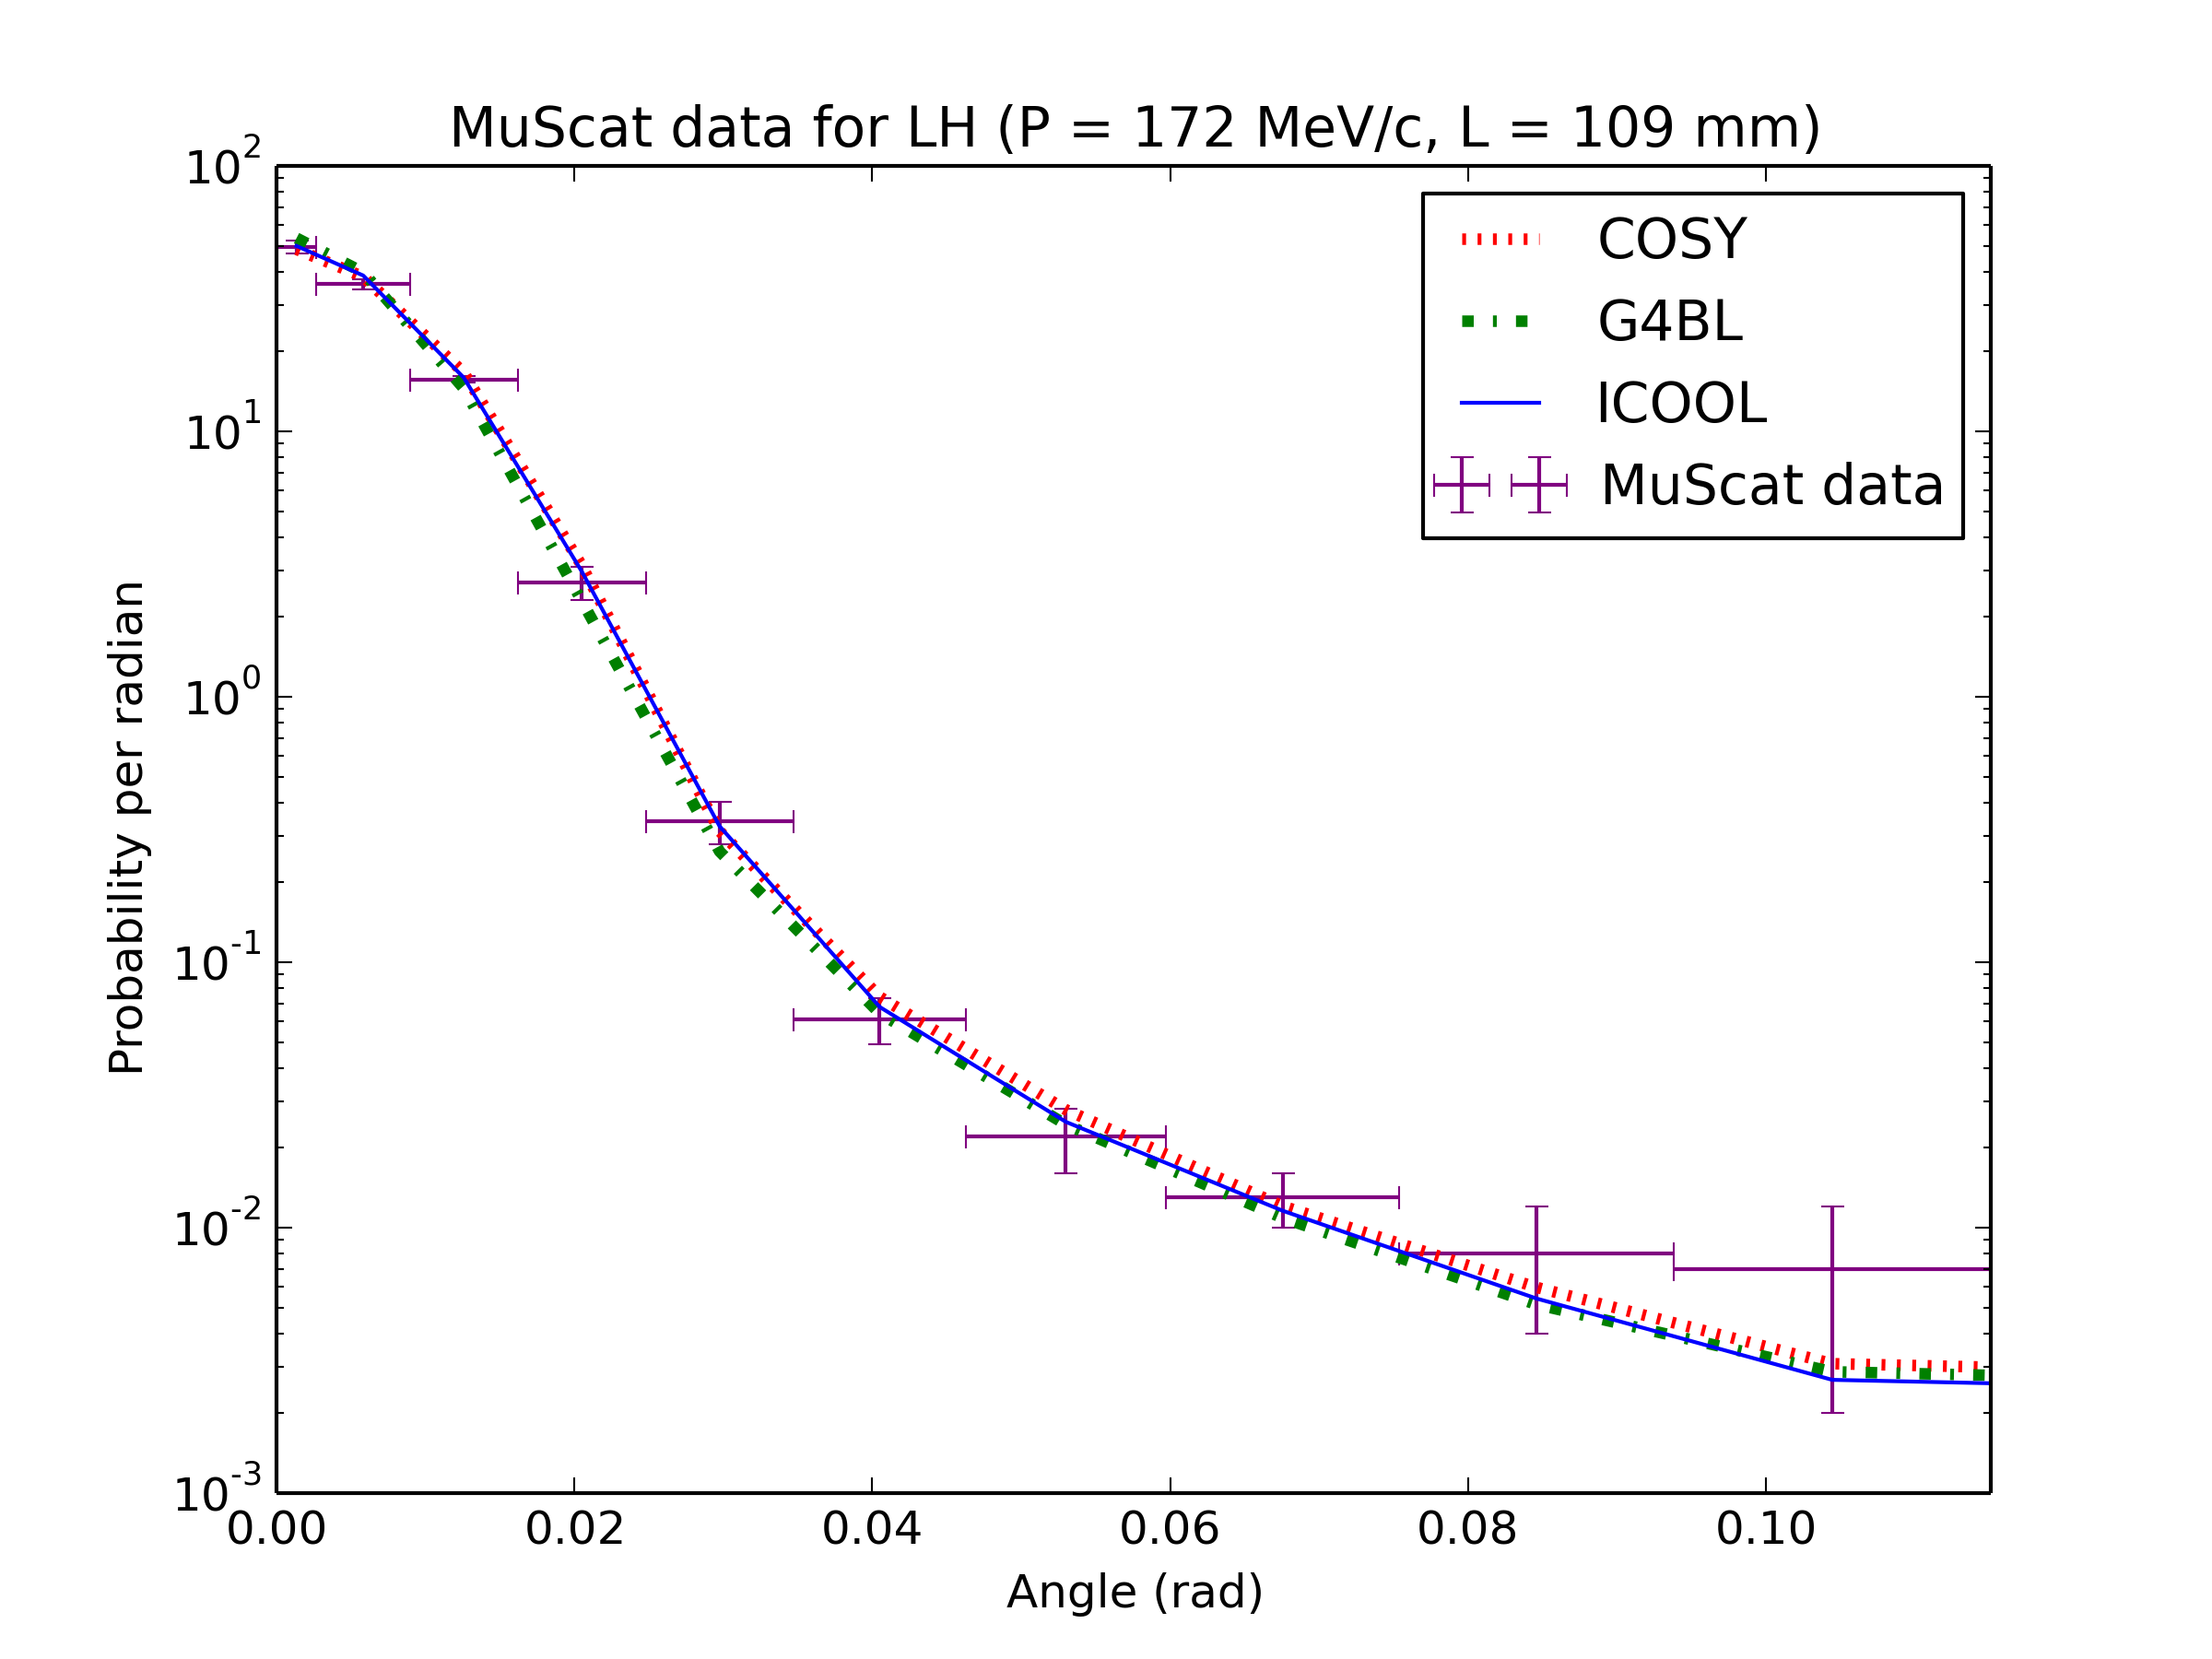
\includegraphics[width=\textwidth]{Figures/172.109.muscat} 
  \caption{MuScat results for 109 mm of liquid hydrogen compared against COSY (red), G4BL (green), and ICOOL (blue).}
  \label{fig:172.109.muscat}
\end{figure}

\begin{figure}[H]
  \centering
    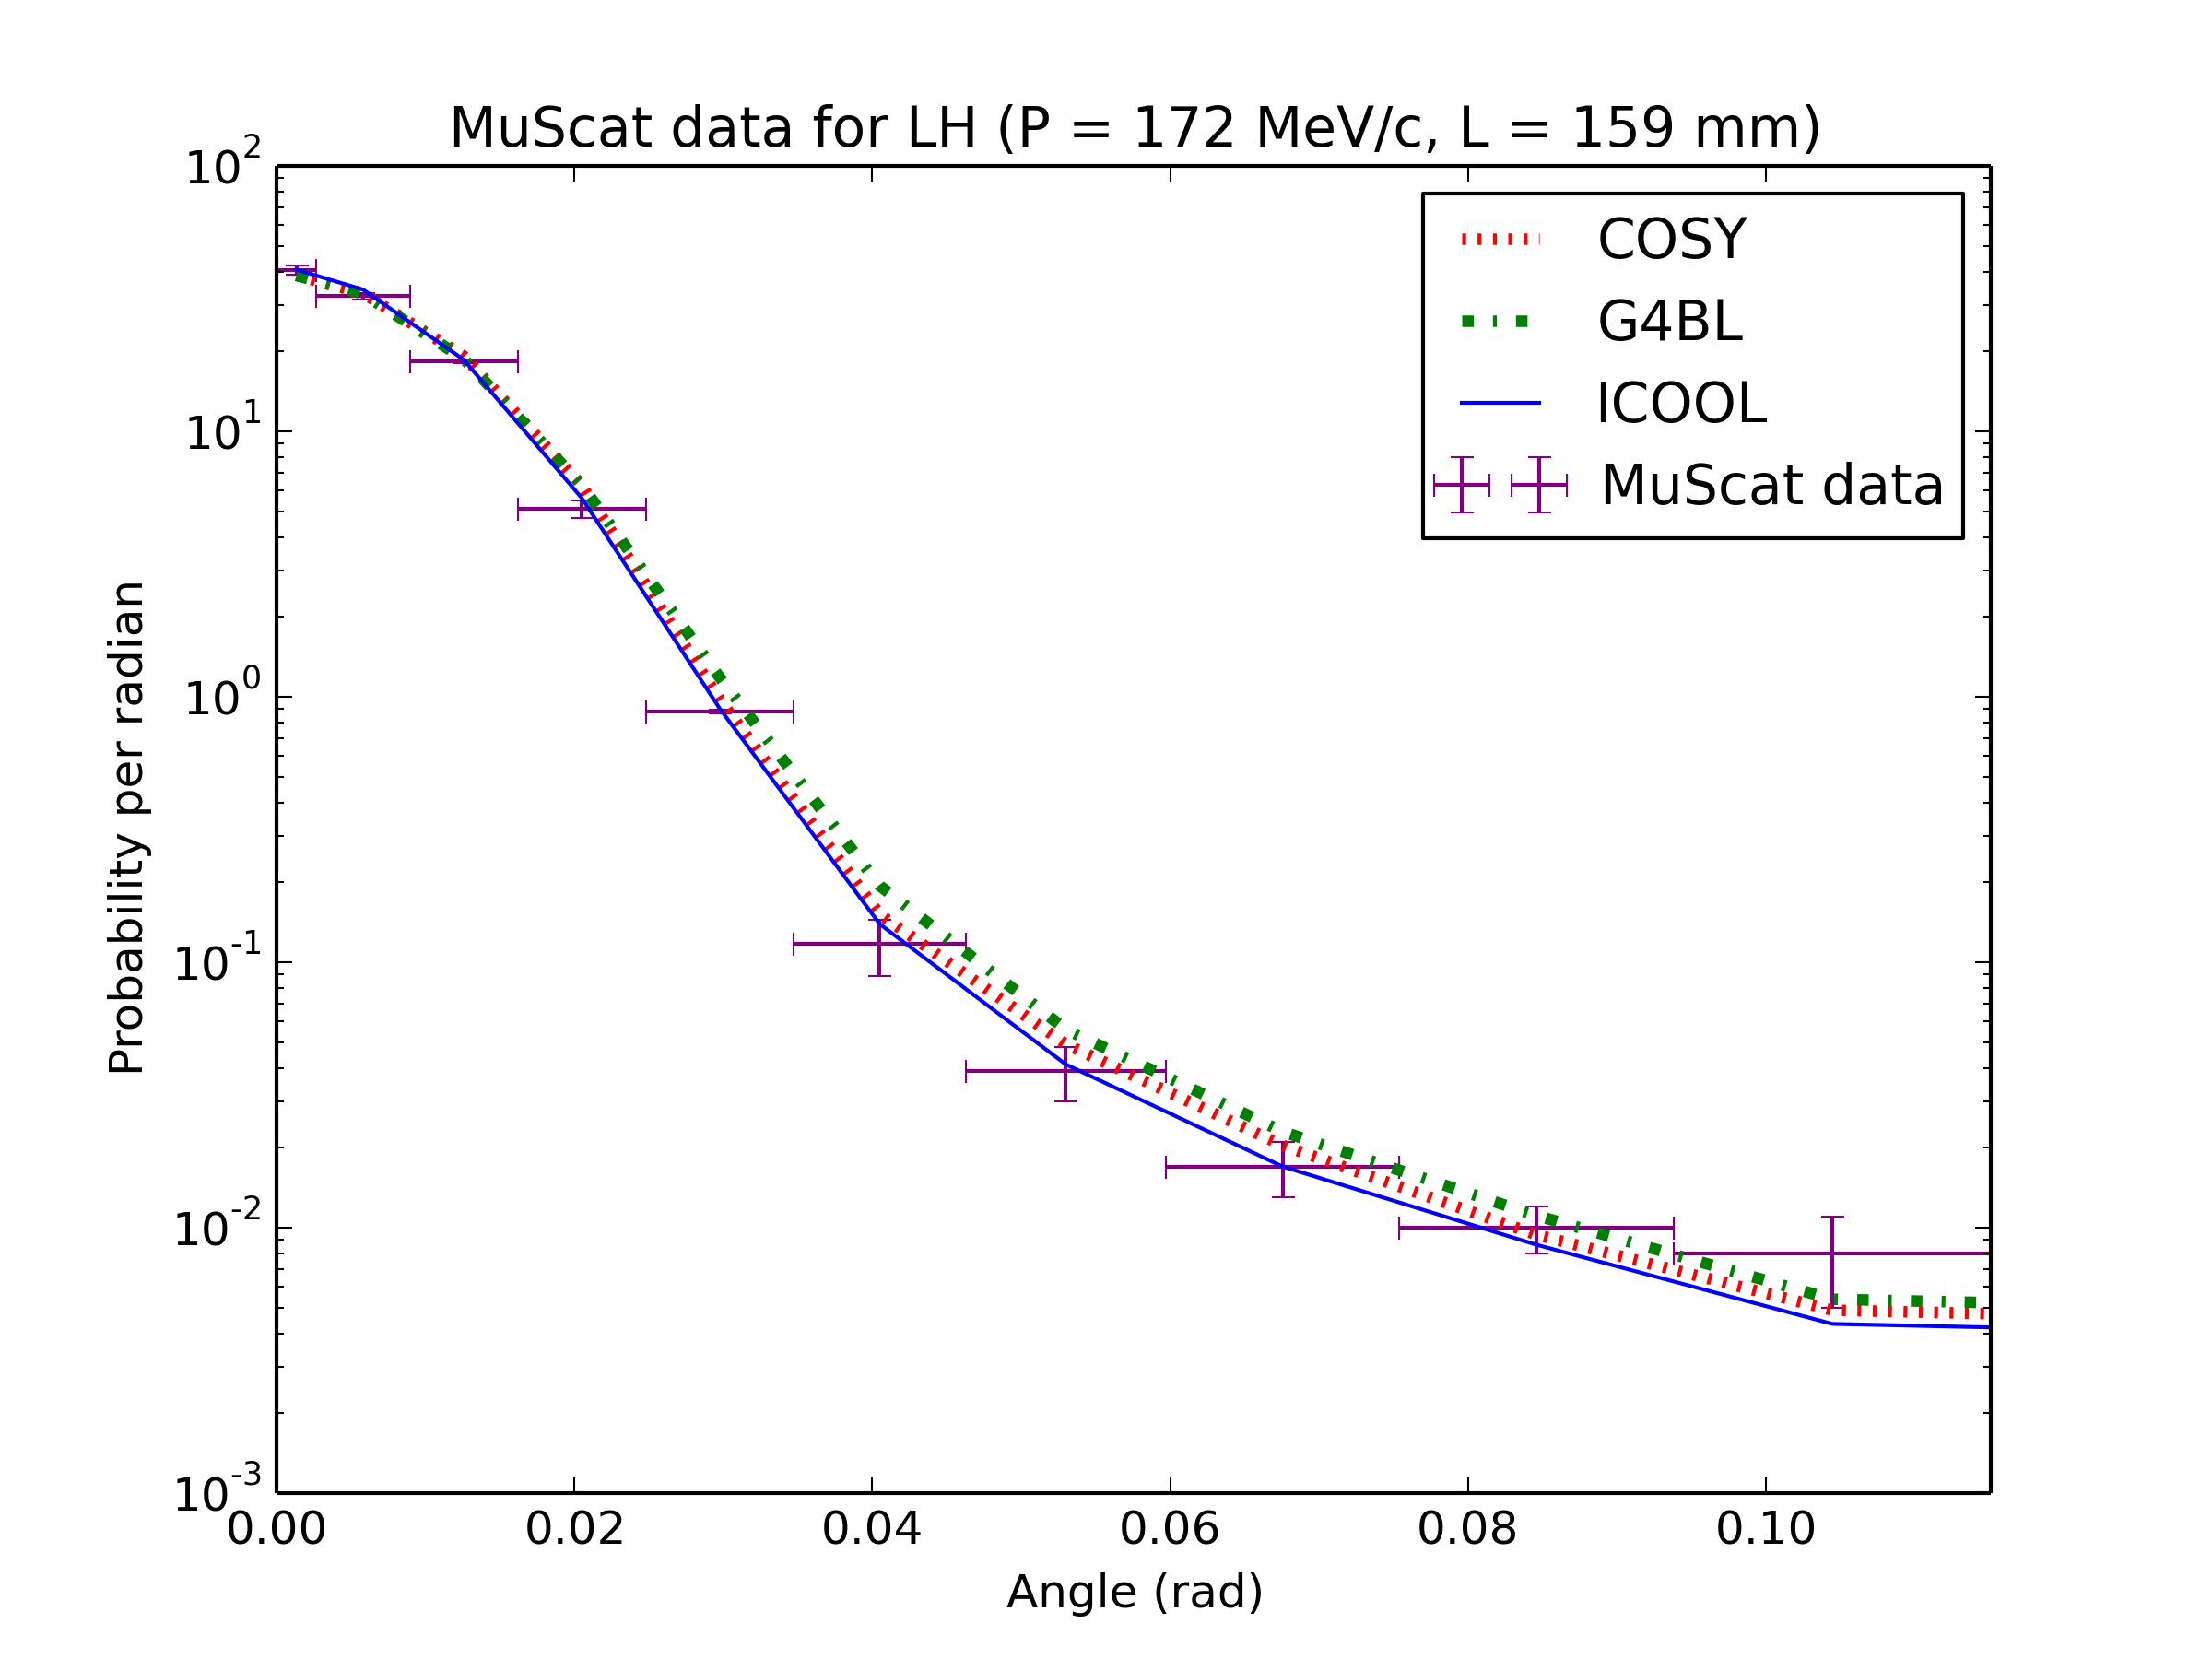
\includegraphics[width=\textwidth]{Figures/172.159.muscat} 
  \caption{MuScat results for 159 mm of liquid hydrogen compared against COSY (red), G4BL (green), and ICOOL (blue).}
  \label{fig:172.159.muscat}
\end{figure}

\begin{figure}[H]
  \centering
    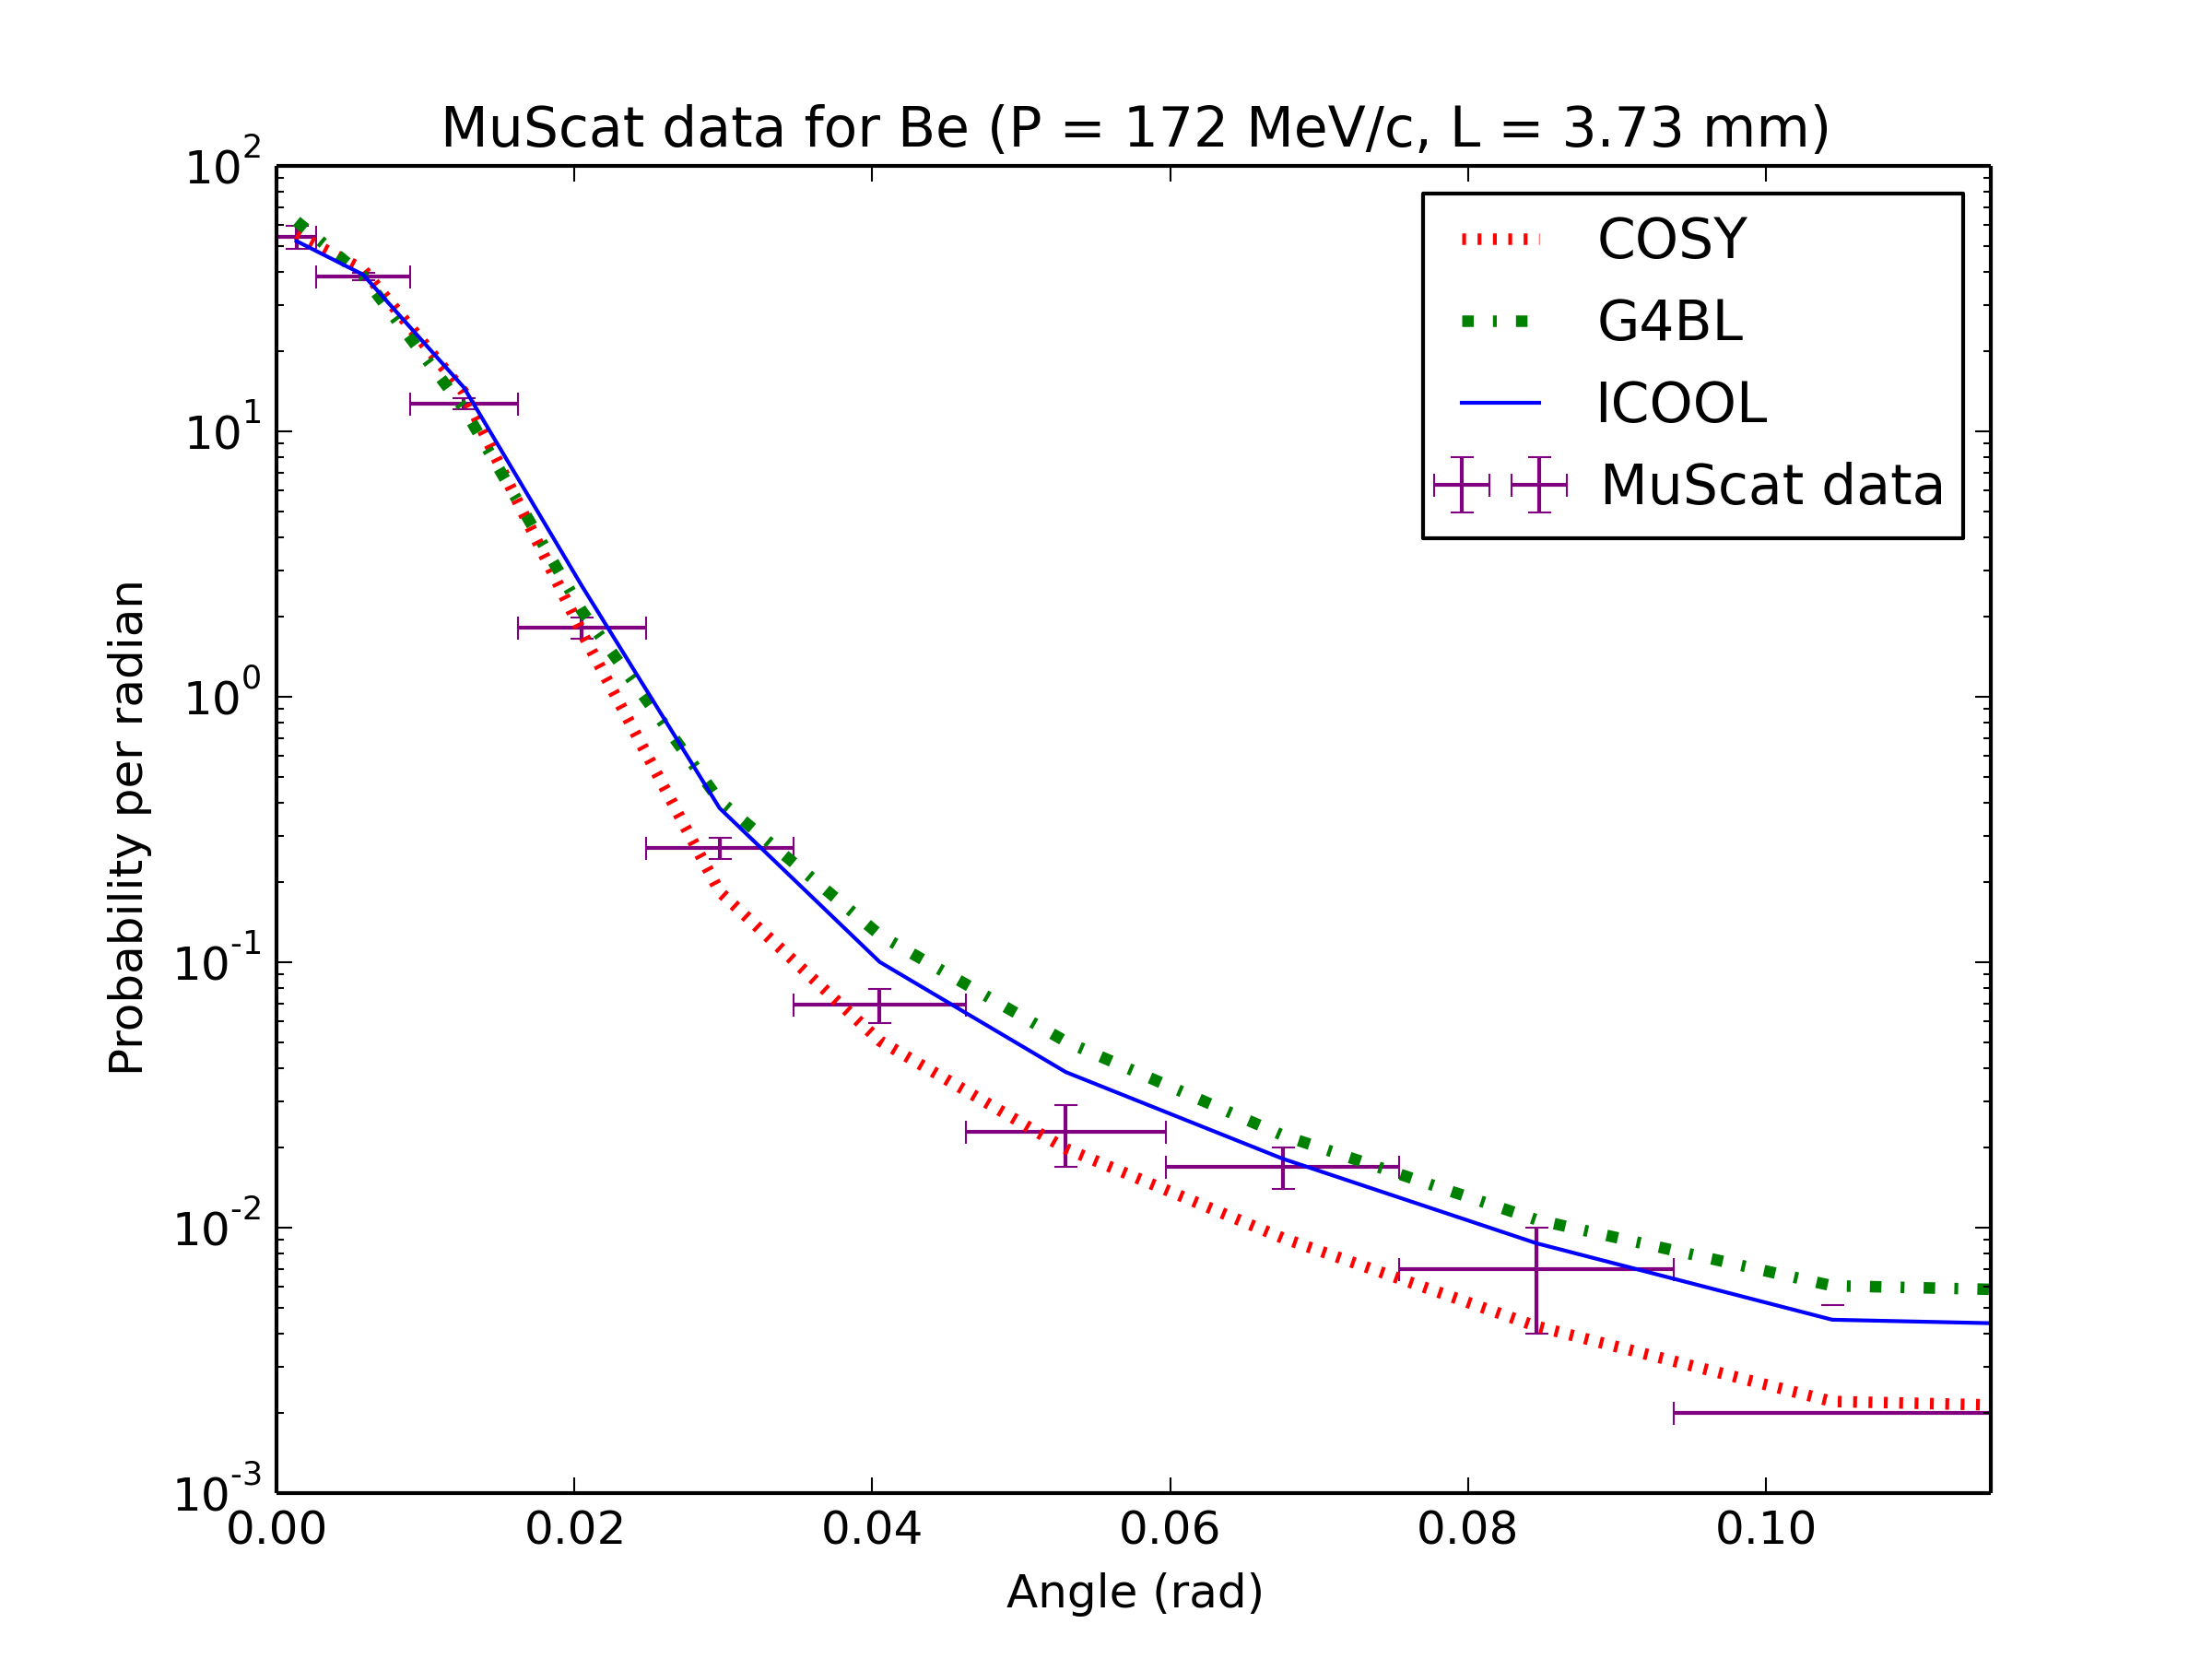
\includegraphics[width=\textwidth]{Figures/172.3.73.muscat} 
  \caption{MuScat results for 3.73 mm of beryllium compared against COSY (red), G4BL (green), and ICOOL (blue).}
  \label{fig:172.3.73.muscat}
\end{figure}

In the liquid hydrogen cases, COSY appears to match both G4Beamline and ICOOL very well, as well as the MuScat data points. ICOOL appears to have a sharper peak than either COSY or G4Beamline, which can be more easily seen in the 159 mm liquid hydrogen case than in the 109 mm case. In the case of beryllium, COSY matches the MuScat points slightly better than G4Beamline and ICOOL, particularly for the two data points between 0.04 and 0.06 radians.

\Section{The Muon Ionization Cooling Experiment}\label{sec:mice}

This section introduces the Muon Ionization Cooling Experiment (MICE, \cite{mice}), a practical application for the new absorber routines in COSY. The results of the MICE simulations in ICOOL, G4Beamline, and COSY will be examined, showing good agreement.

\Subsection{Introduction to MICE}\label{ssc:miceIntro}
The Muon Ionization Cooling Experiment (MICE \cite{mice}) is an experiment currently being developed at the Rutherford Appleton Laboratory in Oxfordshire, U.K. Its goal is to show a proof-of-principle demonstration of muon ionization cooling. While there are six steps, the MICE Step IV configuration is explored in this work. The Step IV cell includes 12 magnetic coils positioned symmetrically around a flat absorber. Figure \ref{fig:miceStepIV} shows a schematic of this lattice with 350 mm of liquid hydrogen as the absorber.
\begin{figure}[h!]
  \centering
    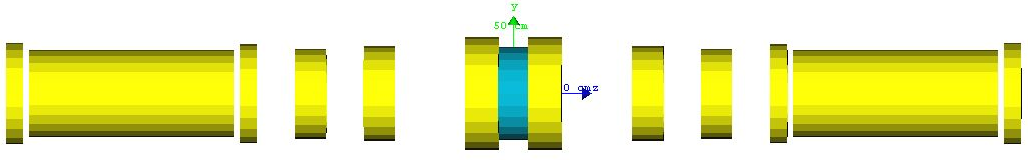
\includegraphics[width=\textwidth]{Figures/miceStepIV} 
  \caption[MICE Step IV cell.]{MICE Step IV cell. Magnetic coils are shown in yellow and the absorber is shown in blue. The green and blue axes are the $y$ and $z$ axes, here drawn to scale as 50 cm each. Image rendered via G4Beamline \cite{g4bl}.}
  \label{fig:miceStepIV}
\end{figure}

\Subsection{Results of the MICE Simulation}\label{ssc:miceResults}
$10^6$ muons were simulated through the cell in Figure \ref{fig:miceStepIV}. The coil parameters may be found in Table \ref{tbl:MICE_coil_parameters}. The absorber was a 350 mm cylindrical block of liquid hydrogen centered at $z=0$. The decay process was disabled in all simulation codes. The beam started at $-$2.45105 m and ended at 2.450 m. The Gaussian parameters for the initial distribution of particles can be found in Table \ref{tbl:MICE_initial_distribution_parameters}.

\begin{table}
\caption*{\textbf{MICE Step IV Coil Parameters}}
\begin{tabularx}{\textwidth}{cccccccc}
\hline \hline
Name & $z$ position & Length & Inner radius & Outer radius & Current density  \vspace{-12pt}\\
 & mm & mm & mm & mm & A/mm$^2$  \\
\hline
	End2 & $\mp$3200.28&110.642&258&325.783&$\pm$126 \vspace{-12pt}\\
	Center&$\mp$2450.275&1314.3&258&280.125&$\pm$148 \vspace{-12pt}\\
	End1 & $\mp$1700.29& 110.642& 258 & 318.905 & $\pm$133 \vspace{-12pt}\\
	Match2 & $\mp$1300.29 & 199.492 & 258 & 288.925 & $\pm$132 \vspace{-12pt}\\
	Match1 & $\mp$860.645 & 201.268 & 258 & 304.165 & $\pm133$ \vspace{-12pt}\\
	Focus & $\mp$202.2 & 213.3 & 267.6 & 361.9 & $\pm$104 \\ 
\hline
\end{tabularx}
\caption[MICE Step IV coil parameters.]{MICE Step IV coil parameters corresponding to Figure \ref{fig:miceStepIV}.}
\label{tbl:MICE_coil_parameters}
\end{table}

%\newcolumntype{A}{ >{\centering\arraybackslash} m{2.5cm} } 
\begin{table}
\caption*{\textbf{MICE Step IV Initial Distribution Parameters}}
\begin{center}
\begin{tabularx}{0.7\textwidth}{p{1cm}ccc}
\hline \hline
&Parameter & Mean & Standard deviation \\
\hline
	&$x$ (mm) & 0 & 32\vspace{-12pt}\\
	&$y$ (mm) & 0 & 32\vspace{-12pt} \\
	&$z$ (mm) & 0 & 0\vspace{-12pt} \\
	&$p_x$ (MeV/$c$) & 0 & 20\vspace{-12pt} \\
	&$p_y$ (MeV/$c$) & 0 & 20\vspace{-12pt} \\
	&$p_z$ (MeV/$c$) & 200 & 30\\
\hline
\end{tabularx}
\end{center}
\caption{MICE Step IV initial distribution Gaussian parameters.}
\label{tbl:MICE_initial_distribution_parameters}
\end{table}

For COSY, it was found that a 5th order simulation was sufficient. Through the coil-only portion of the simulation, 100 steps were taken on each side of the absorber (or roughly a step size of 24.5 mm both upstream and downstream). The selection of order and step size will be detailed in the next section. The particles were tracked through the momentary tranfer map after each step and then the transfer map was cleared. It was noted that for the coil-only section, a single transfer map was not sufficient even at the 21st order. This is likely due to the large phase space volume of the initial beam and the complexity of the magnetic field.

Compounding the map without propagating the beam also gave poor results. When one takes the composition of two $n^{th}$ order transfer maps, a transfer map of order $n\times n$ is the result. For example, the first step in the MICE simulation would yield a 3rd order transfer map. Taking the second step would give a new transfer map of order $3\times 3 = 9$. However, since COSY is operating in the 3rd order mode, the new transfer map would not be 9th order, but rather it would be truncated to a 3rd order map. For this reason, the particles were propagated through the momentary transfer map after each step in the simulation.

When the beam entered the region of the absorber, COSY switched to a step size of 10 mm in order to simulate the superposition of the magnetic coils and the absorber.

The magnetic field in G4Beamline was created using the \texttt{coil} and \texttt{solenoid} commands. The field was then exported to a file using the \texttt{pringfield} command so that ICOOL could read and create its own field map via the \texttt{GRID} command operating in \texttt{G43D} mode.

\begin{figure}[H]
  \centering
    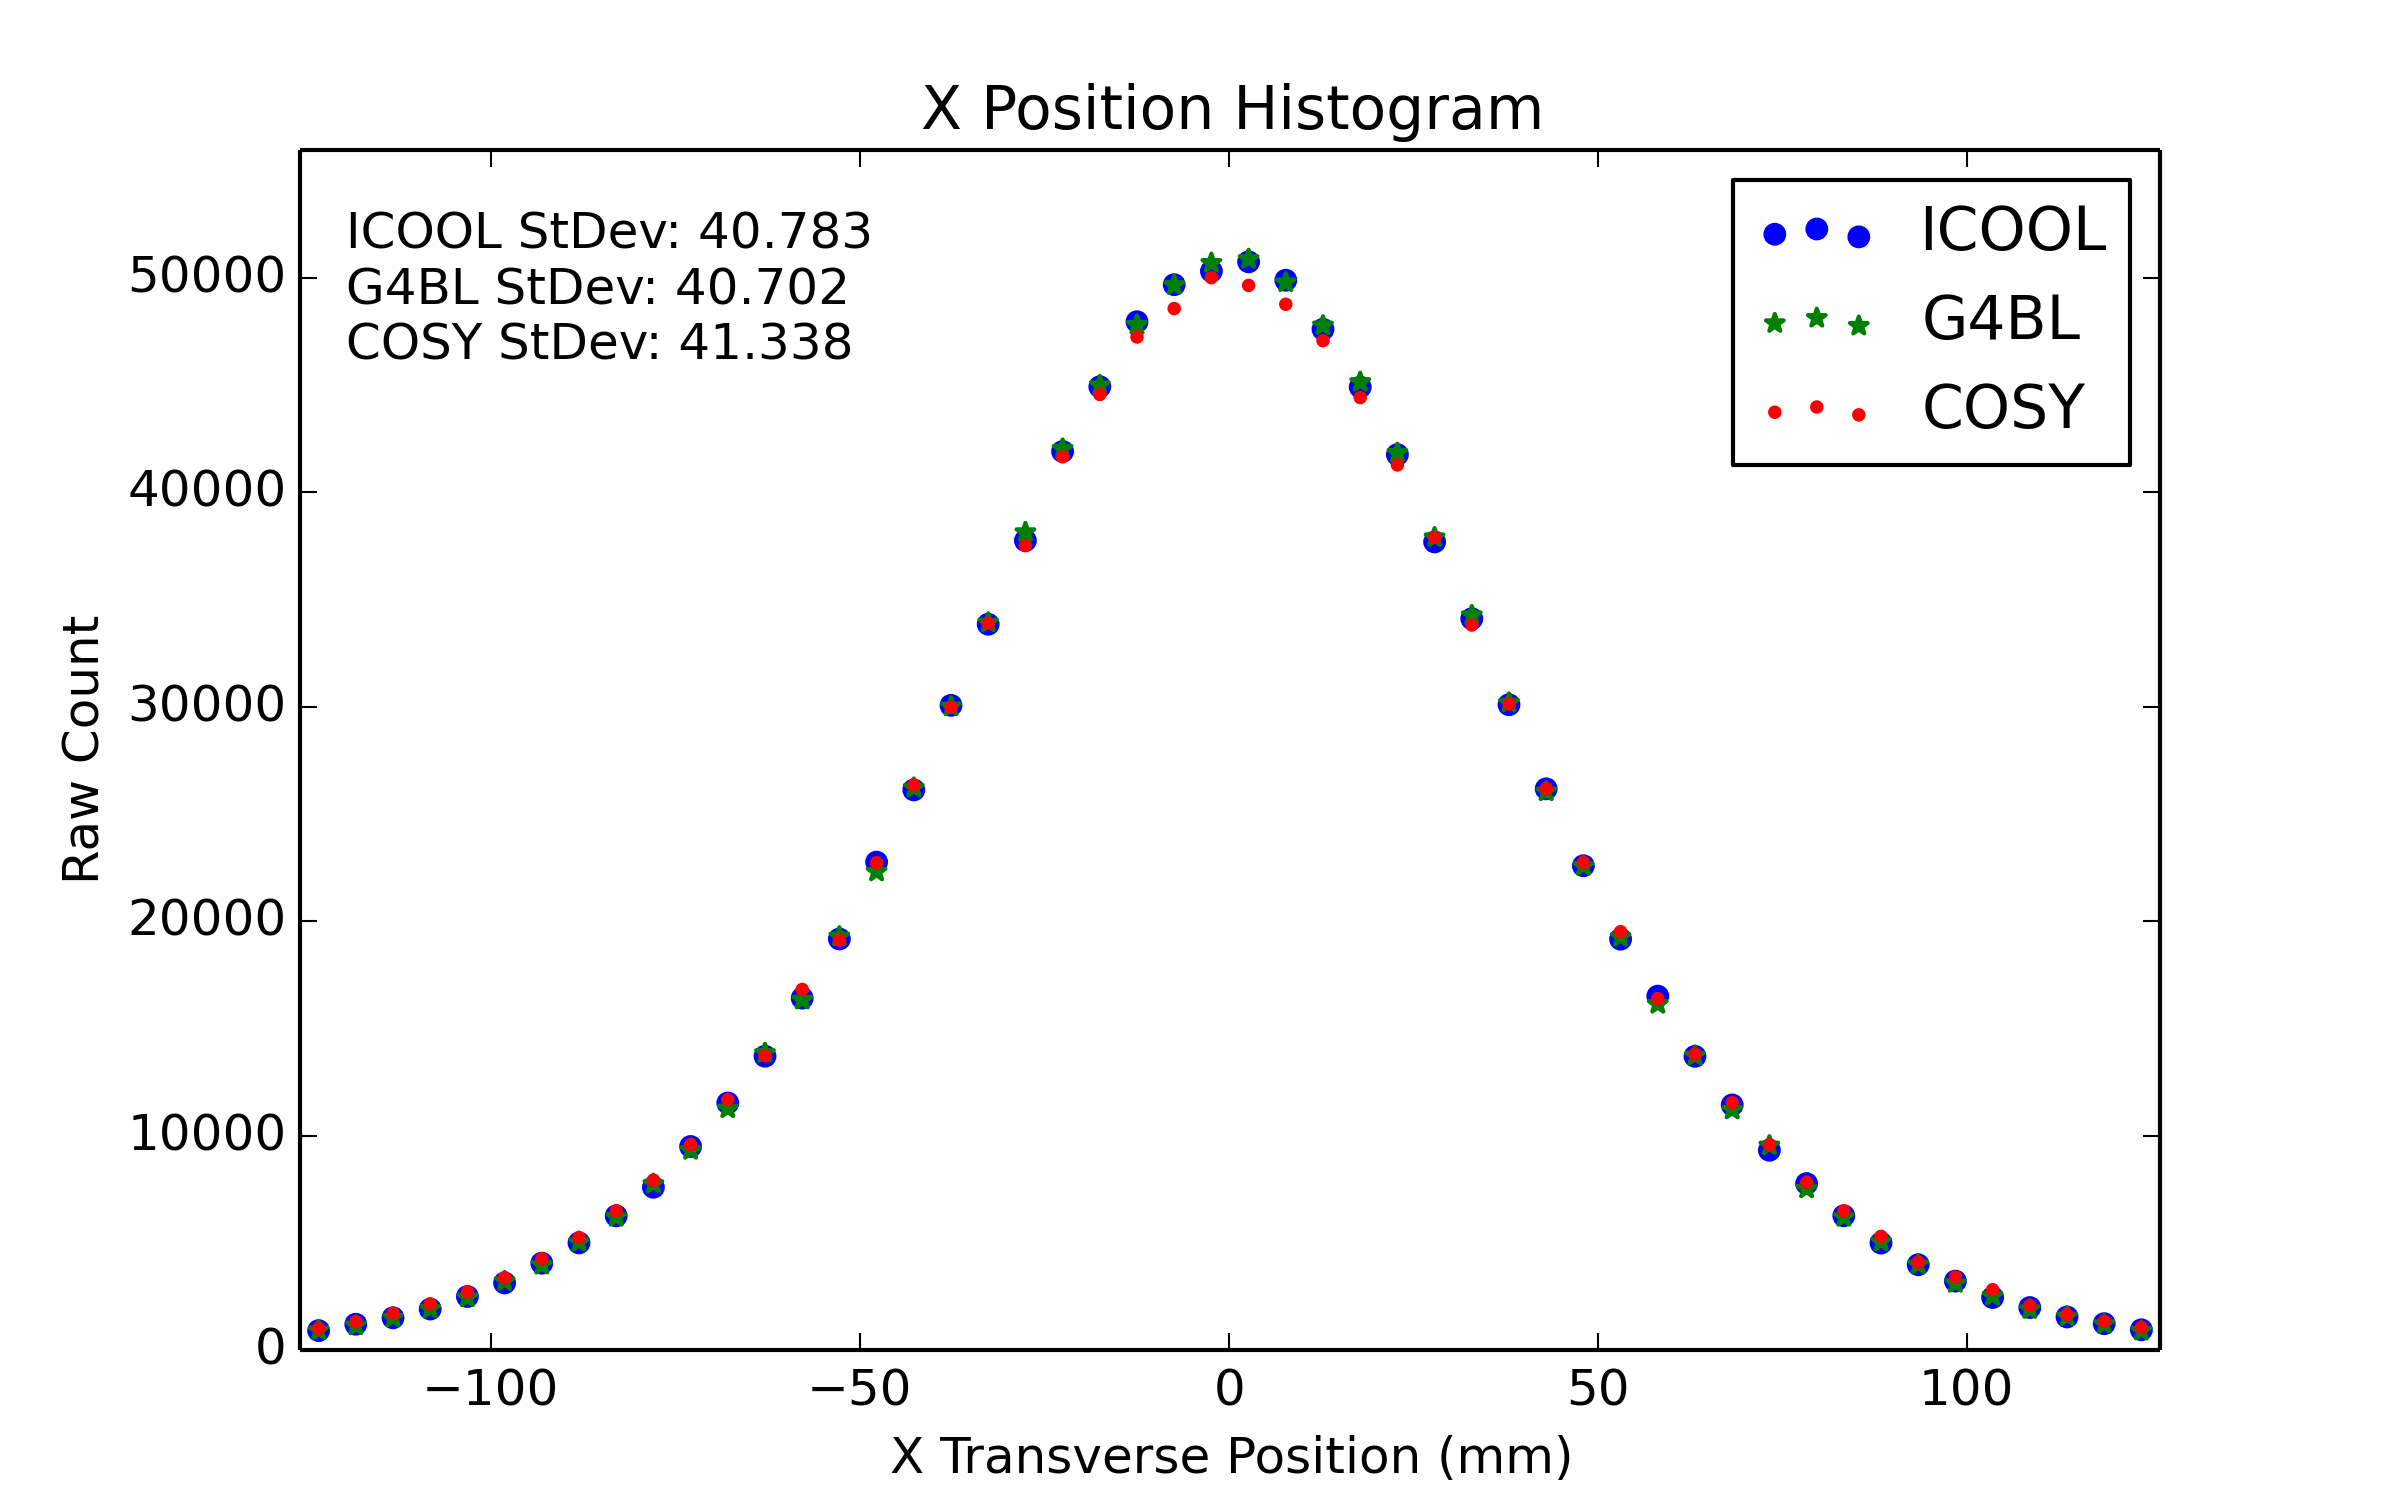
\includegraphics[width=\textwidth]{MICE data/x} 
  \caption{MICE Step IV $x$ position results for liquid hydrogen.}
  \label{fig:micex}
\end{figure}

\begin{figure}[H]
  \centering
    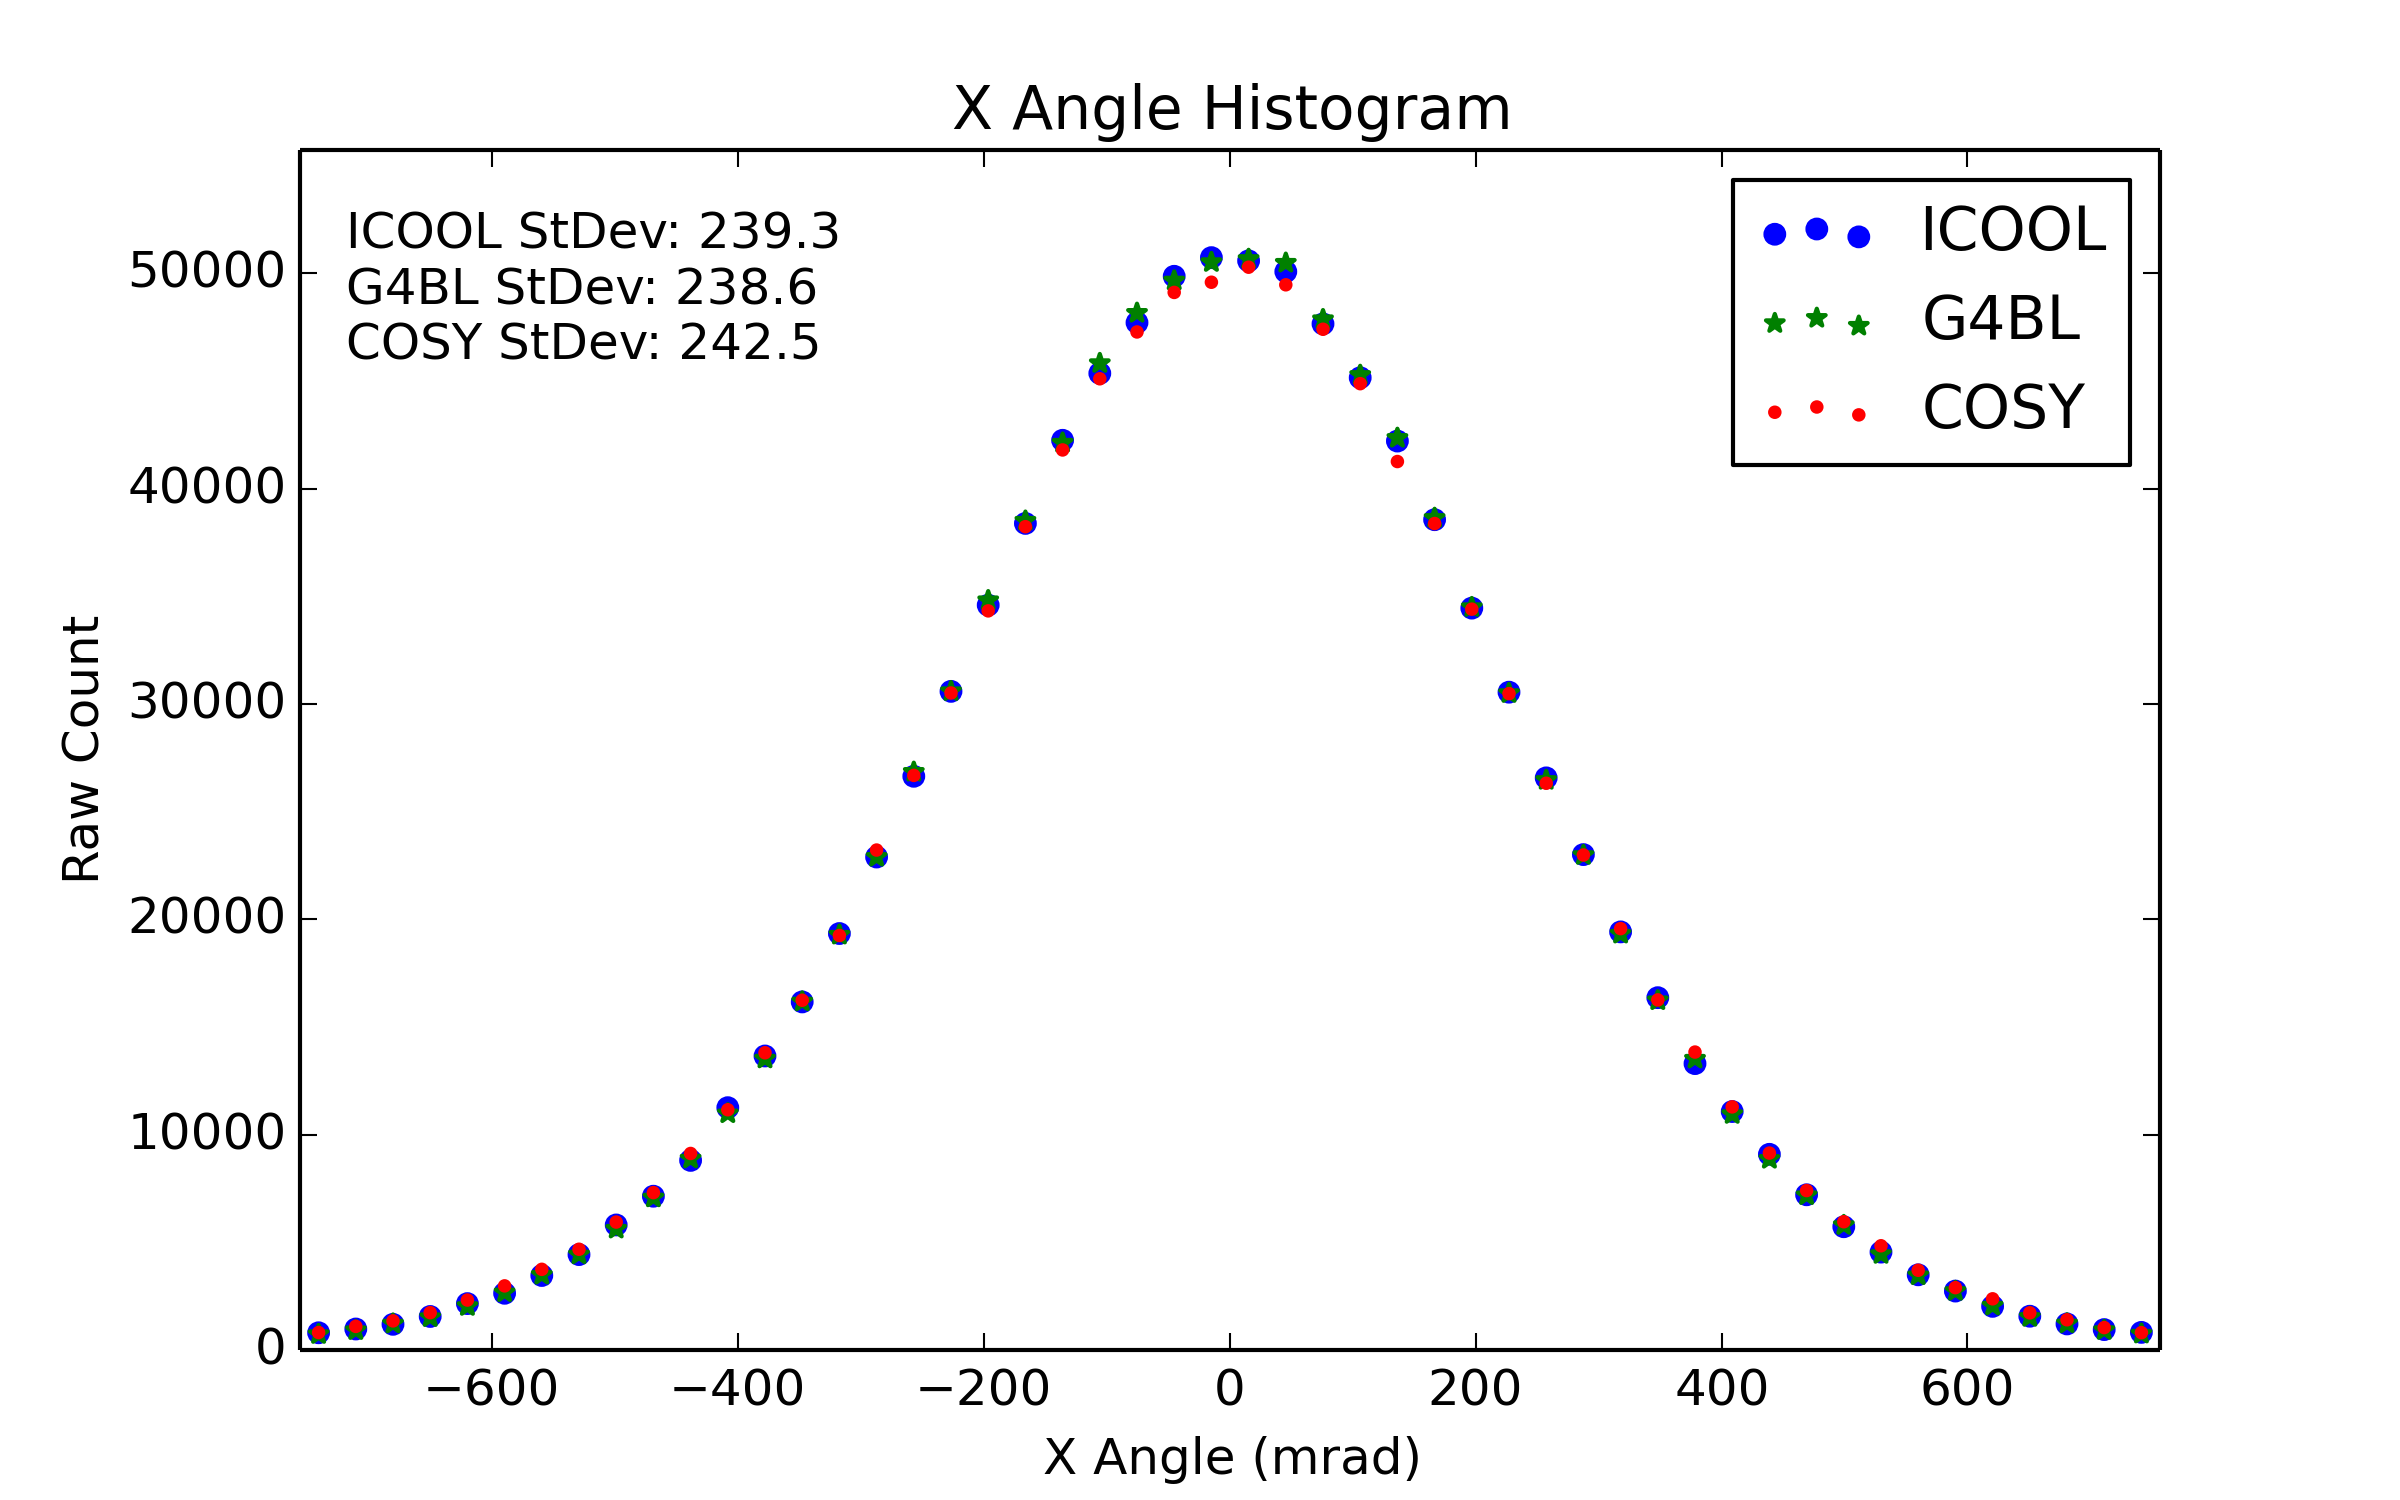
\includegraphics[width=\textwidth]{MICE data/px} 
  \caption{MICE Step IV $x$ angle results for liquid hydrogen.}
  \label{fig:micexangle}
\end{figure}

\begin{figure}[H]
  \centering
    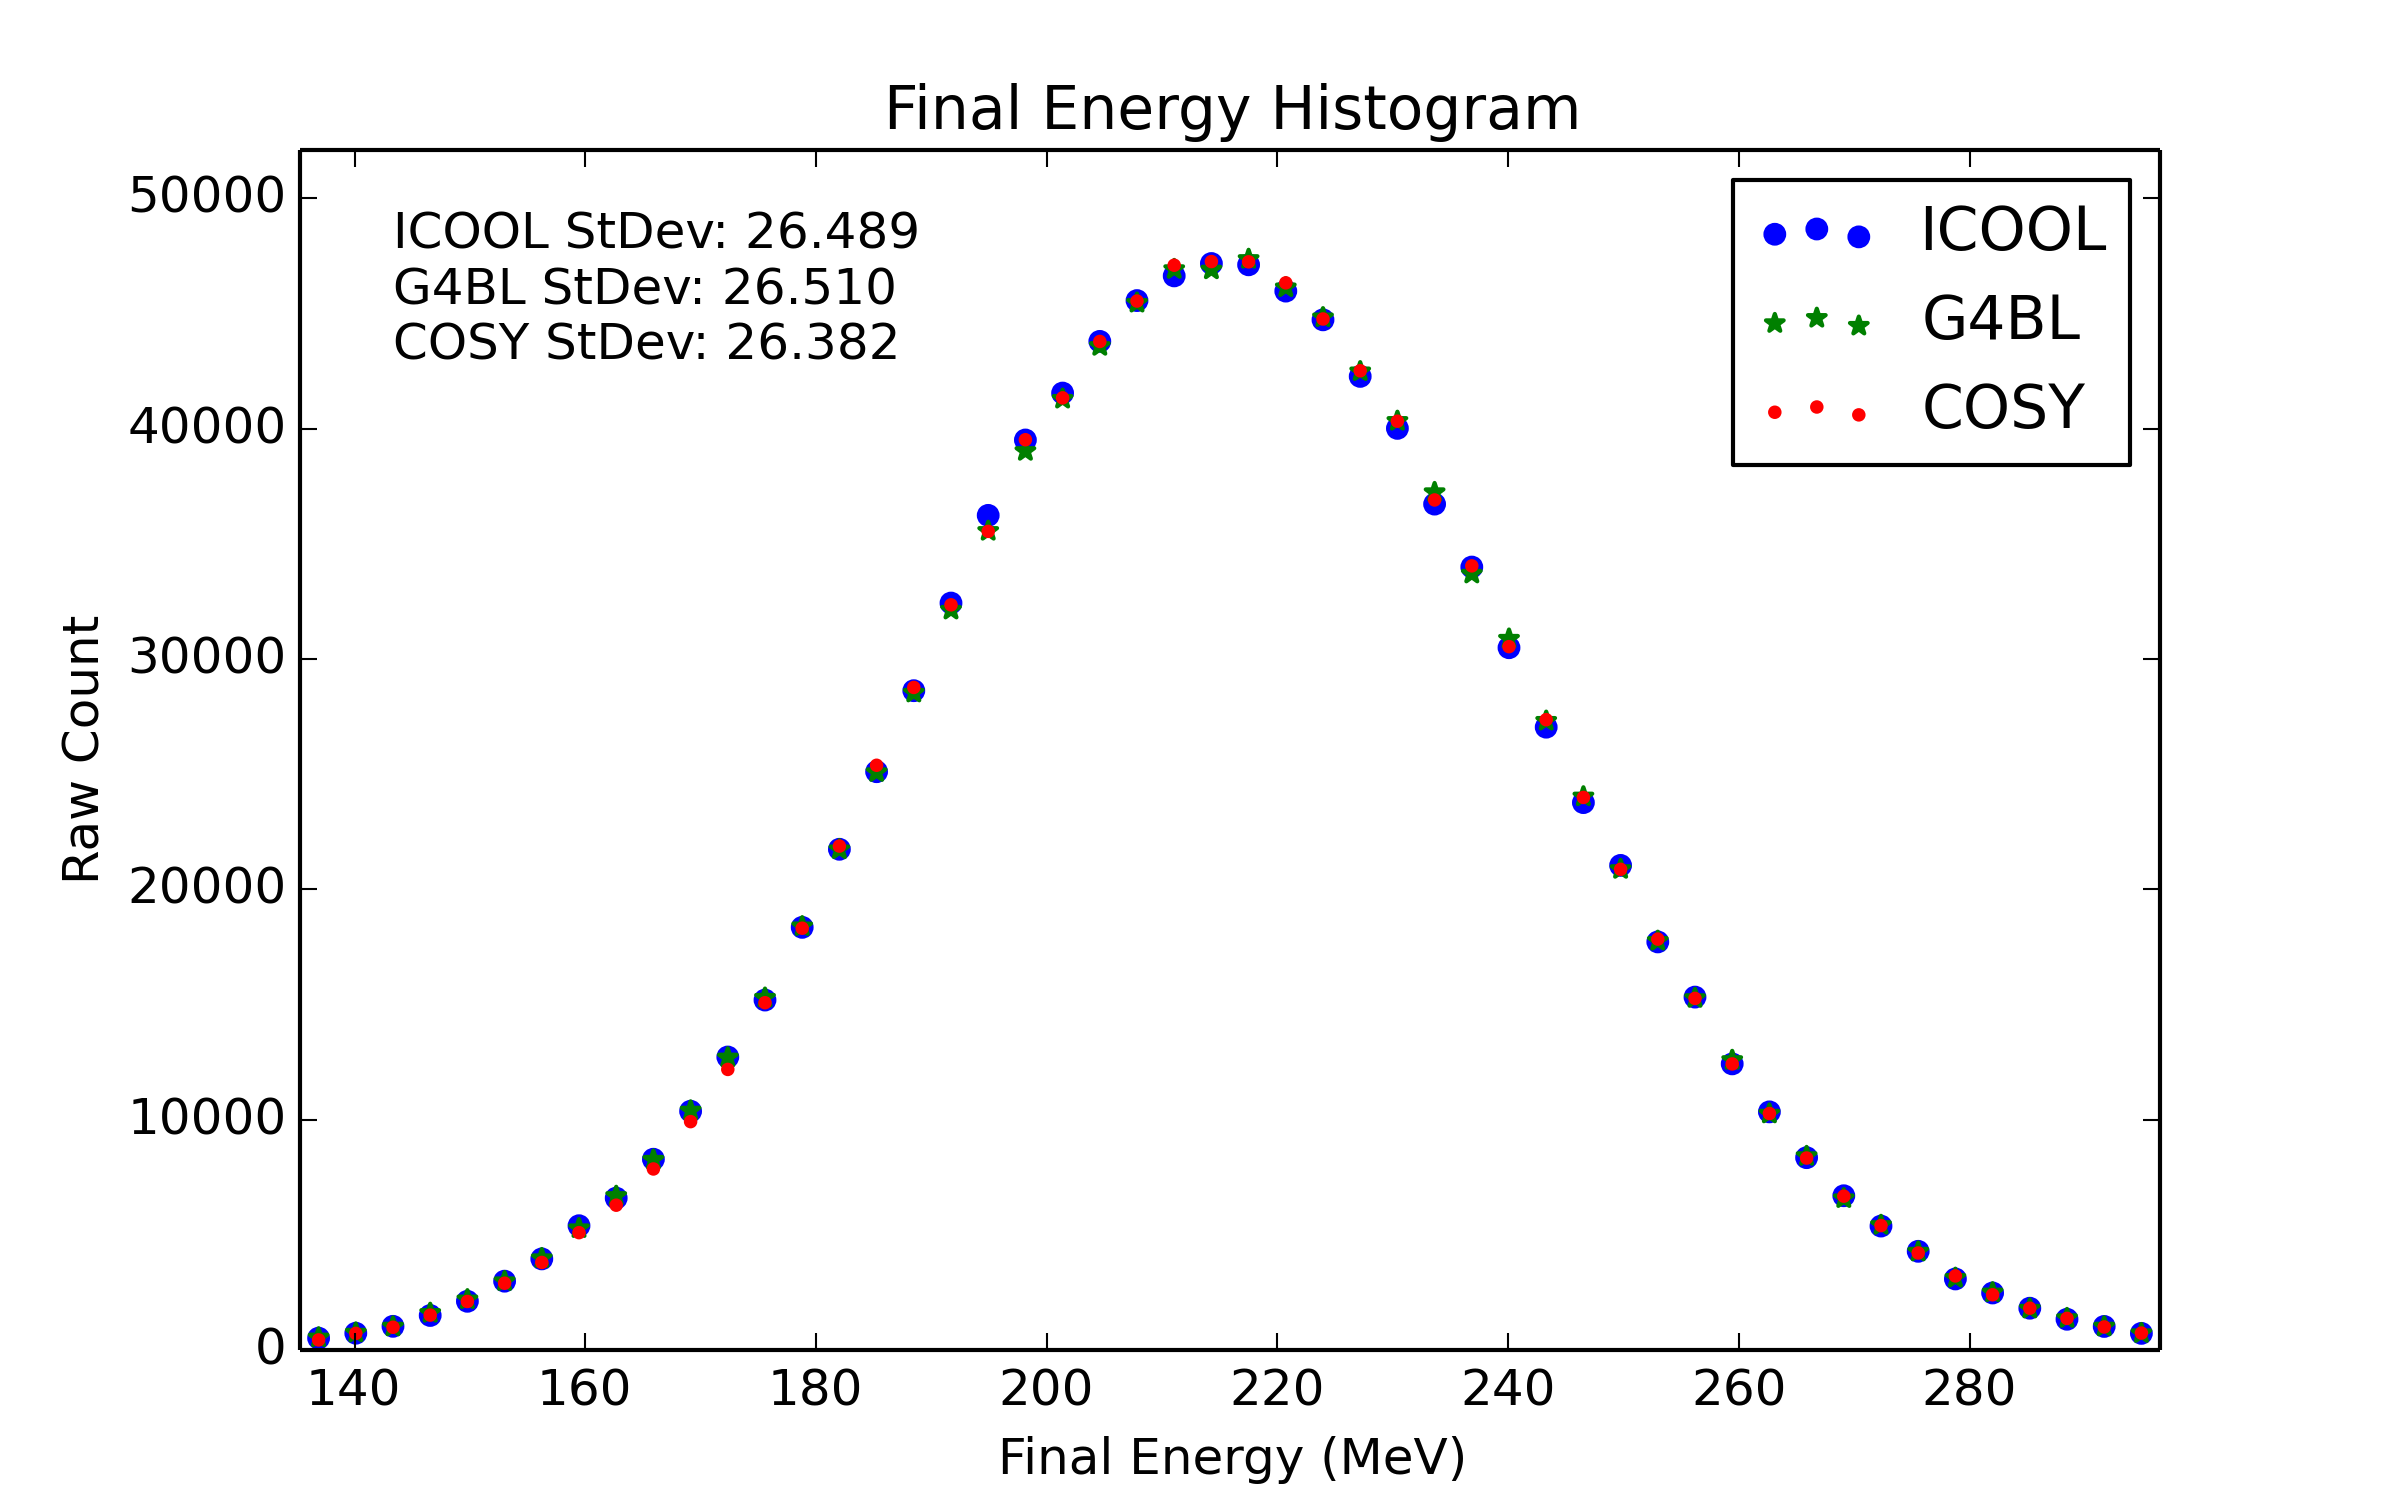
\includegraphics[width=\textwidth]{MICE data/e} 
  \caption{MICE Step IV final energy results for liquid hydrogen.}
  \label{fig:miceenergy}
\end{figure}

The runtimes of ICOOL, G4Beamline, and COSY are listed in Table \ref{tbl:mice_times}. To reiterate, COSY was run at 5th order with 100 steps before the absorber, 350 steps inside the absorber, and 100 steps after the absorber. G4Beamline was left to its default step size. ICOOL was run with a step size of 1 mm. Further note that the initialization time for G4Beamline to create the field maps was 33 seconds. However, since G4Beamline only has to create the field map once the initialization time is not added to the run times in Table \ref{tbl:mice_times}.

\begin{table}
\caption*{\textbf{Run Times (in seconds) for the MICE Step IV Simulation}}
\begin{center}
\begin{tabularx}{0.6\textwidth}{ccccc}
%\vspace{-40pt}\\ 
\hline \hline
Number of particles: & $10^6$ & $10^5$ & $10^4$ & $10^3$\\
\hline
ICOOL: & 27735 & 2655 & 271 & 35\vspace{-12pt}\\
G4Beamline: & 3973 & 392 & 40 & 6\vspace{-12pt}\\
COSY: & 893 & 73 & 13 & 7\\
\hline
\end{tabularx}
\end{center}
\caption[Run Times for the MICE Step IV Simulation.]{Run Times for the MICE Step IV Simulation for liquid hydrogen. Note that the G4Beamline initialization time was not added to the run time values.}
\label{tbl:mice_times}
\end{table}

As a second test, the MICE configuration in Figure \ref{fig:miceStepIV} was simulated using 65 mm of lithium hydride. Lithium hydride is an attractive material because, unlike liquid hydrogen, it does not require cryogenic conditions, but still maintains a low $Z$ value. It can be seen from Figures \ref{fig:mice_lih_x}, \ref{fig:mice_lih_xangle}, and \ref{fig:mice_lih_energy} that 65 mm of lithium hydride has a similar effect on the beam as 350 mm of liquid hydrogen. It should be noted that inside the absorber, a 5 mm step size was chosen instead of a 10 mm step size (since 10 does not evenly go into 65).

\begin{figure}[H]
  \centering
    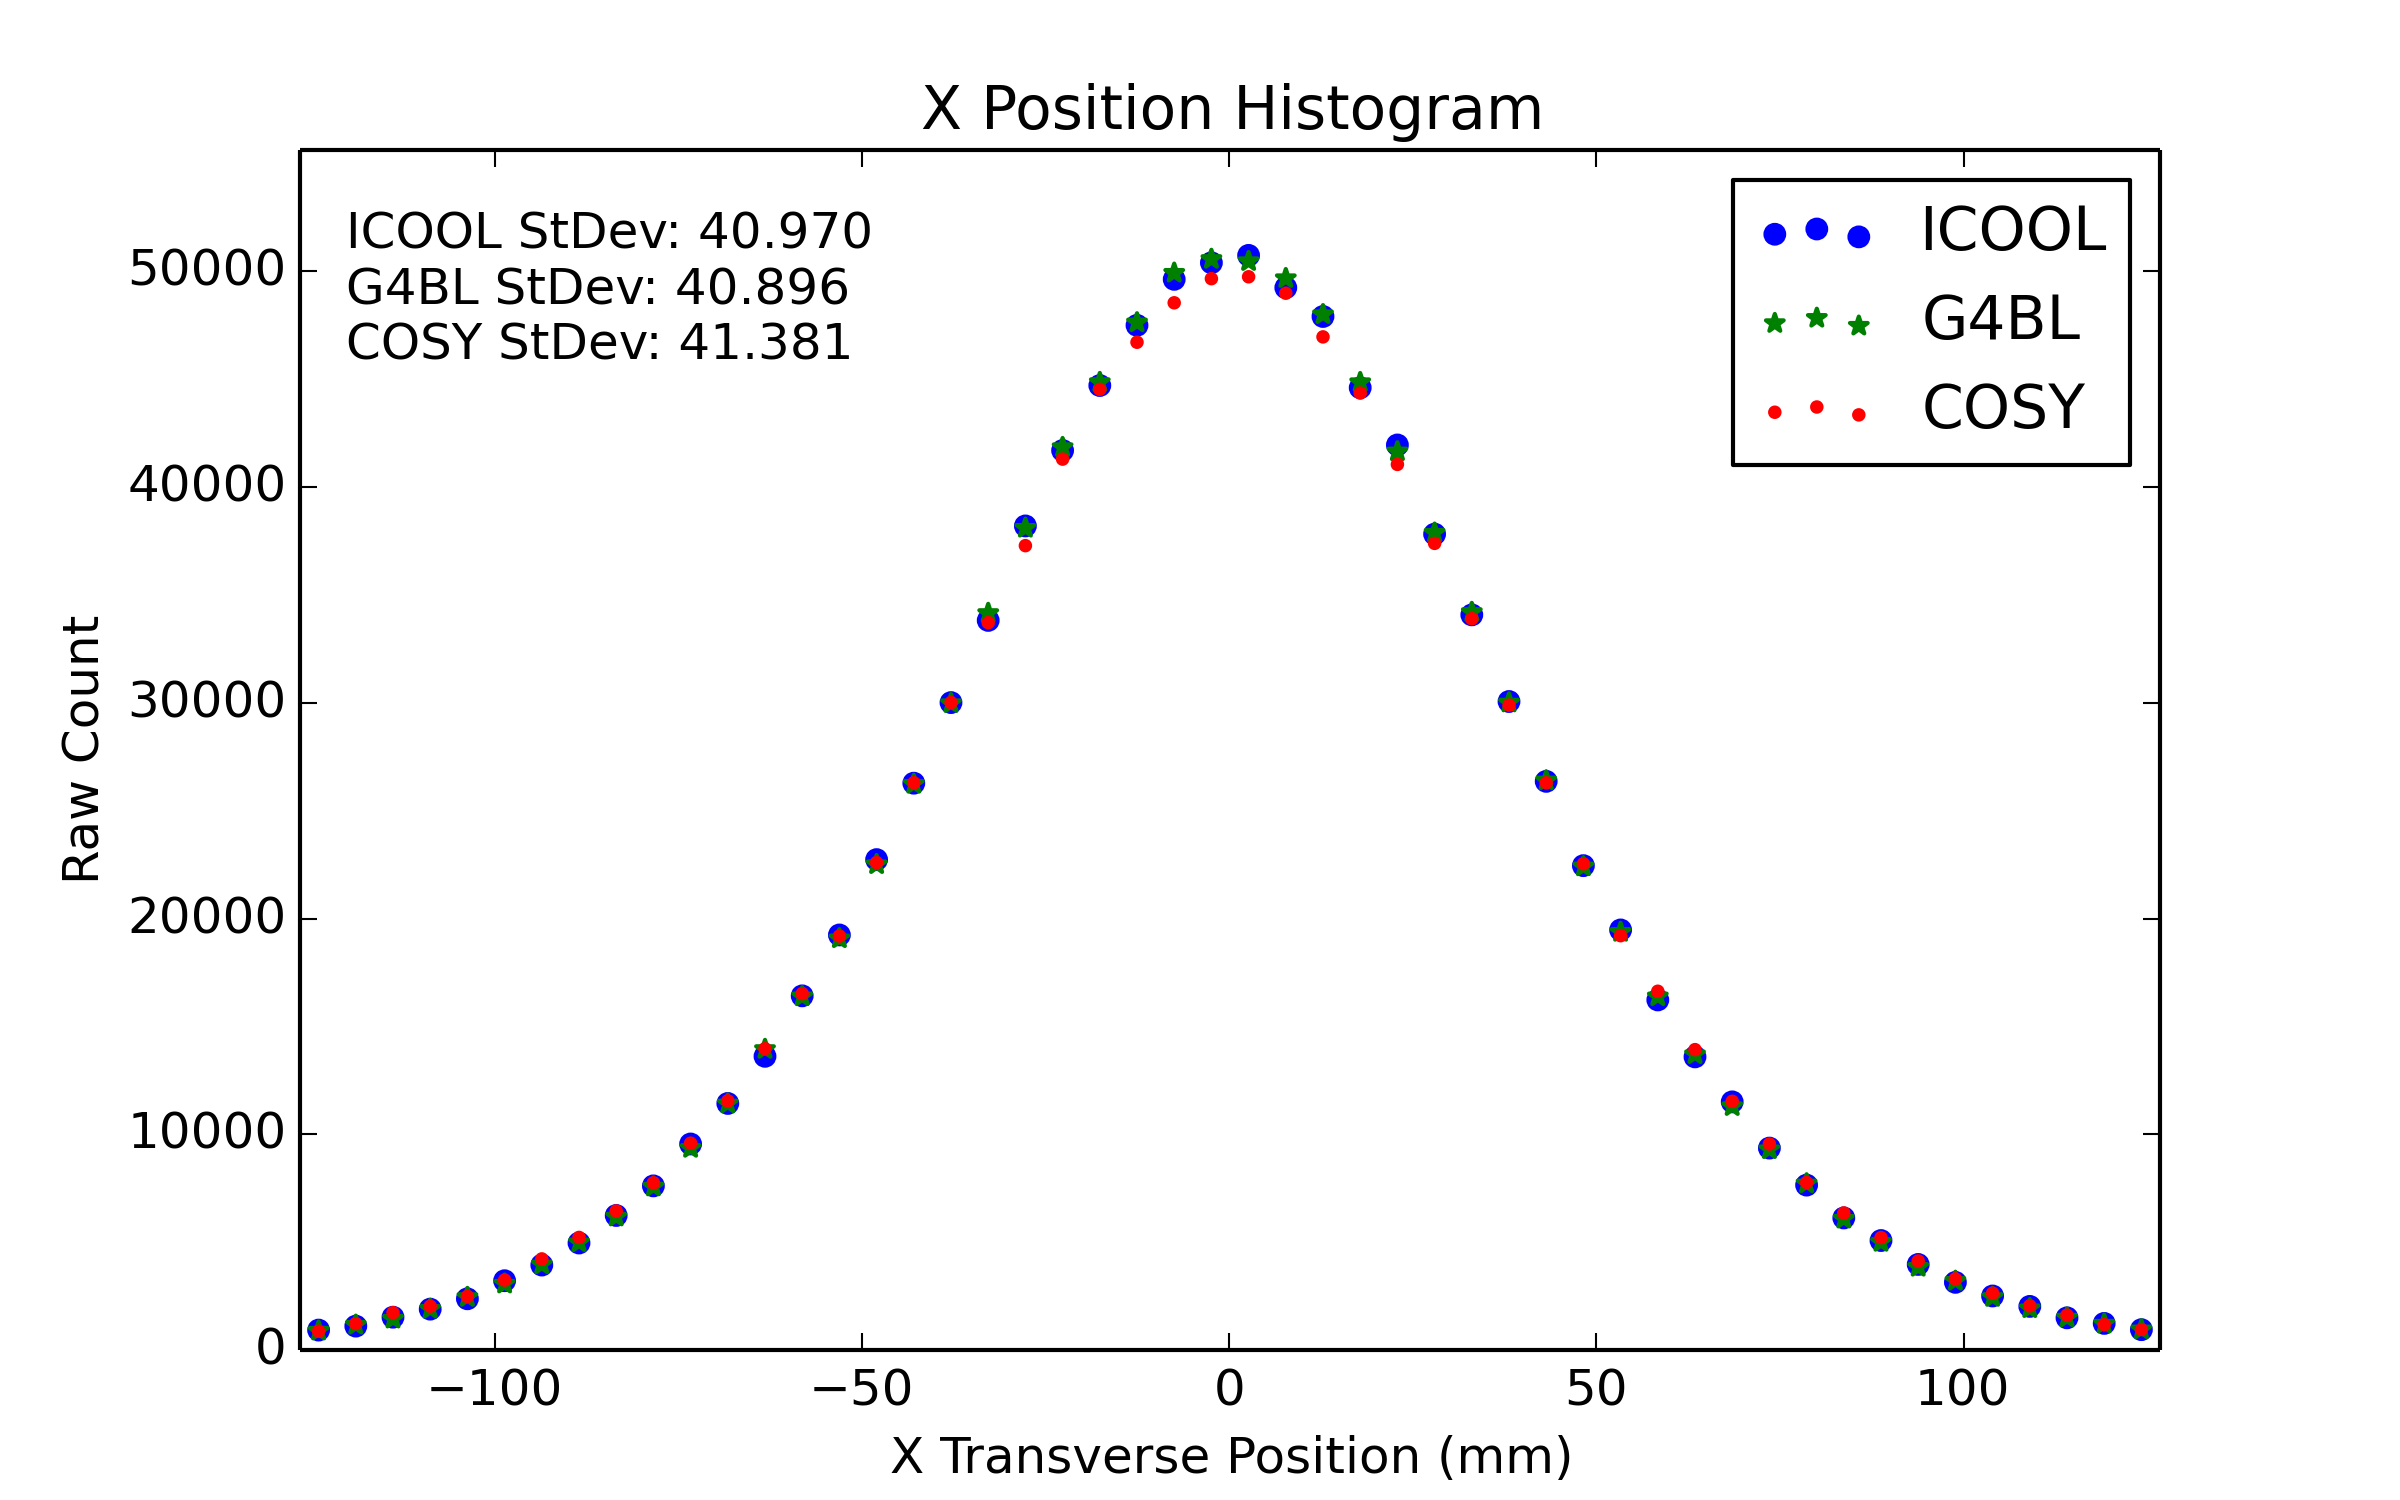
\includegraphics[width=\textwidth]{MICE data/LiH/x} 
  \caption{MICE Step IV $x$ position results for lithium hydride.}
  \label{fig:mice_lih_x}
\end{figure}

\begin{figure}[H]
  \centering
    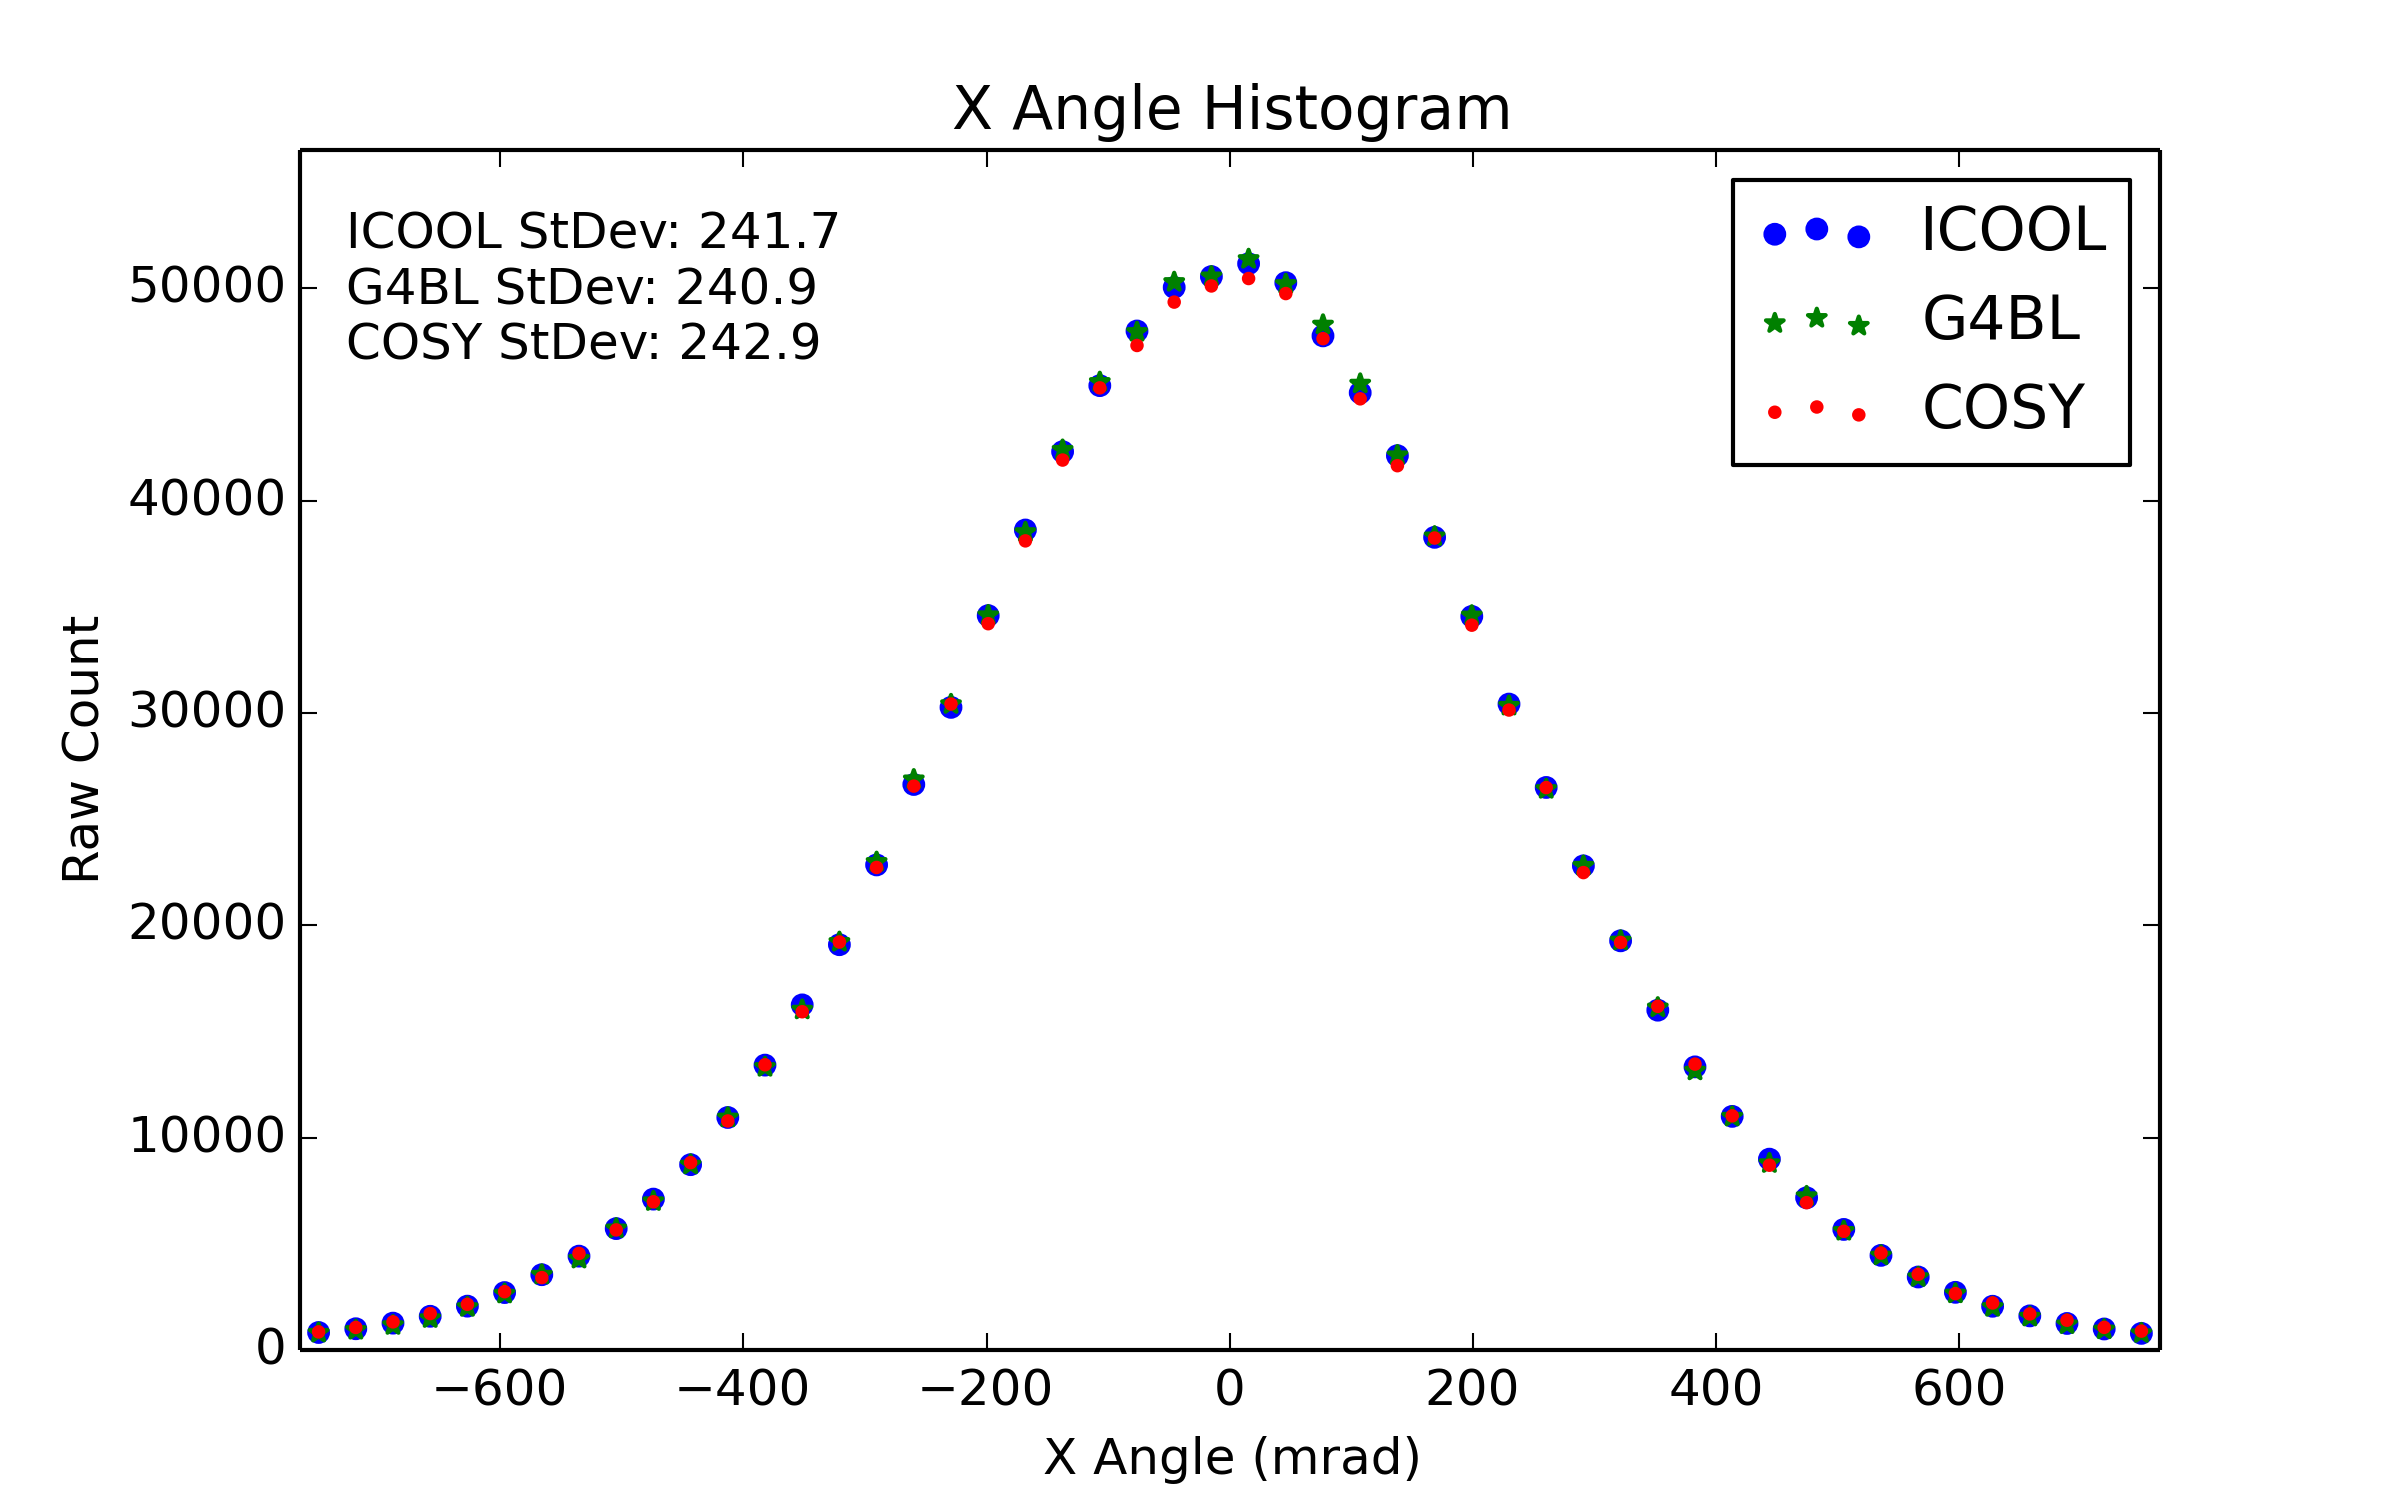
\includegraphics[width=\textwidth]{MICE data/LiH/px} 
  \caption{MICE Step IV $x$ angle results for lithium hydride.}
  \label{fig:mice_lih_xangle}
\end{figure}

\begin{figure}[H]
  \centering
    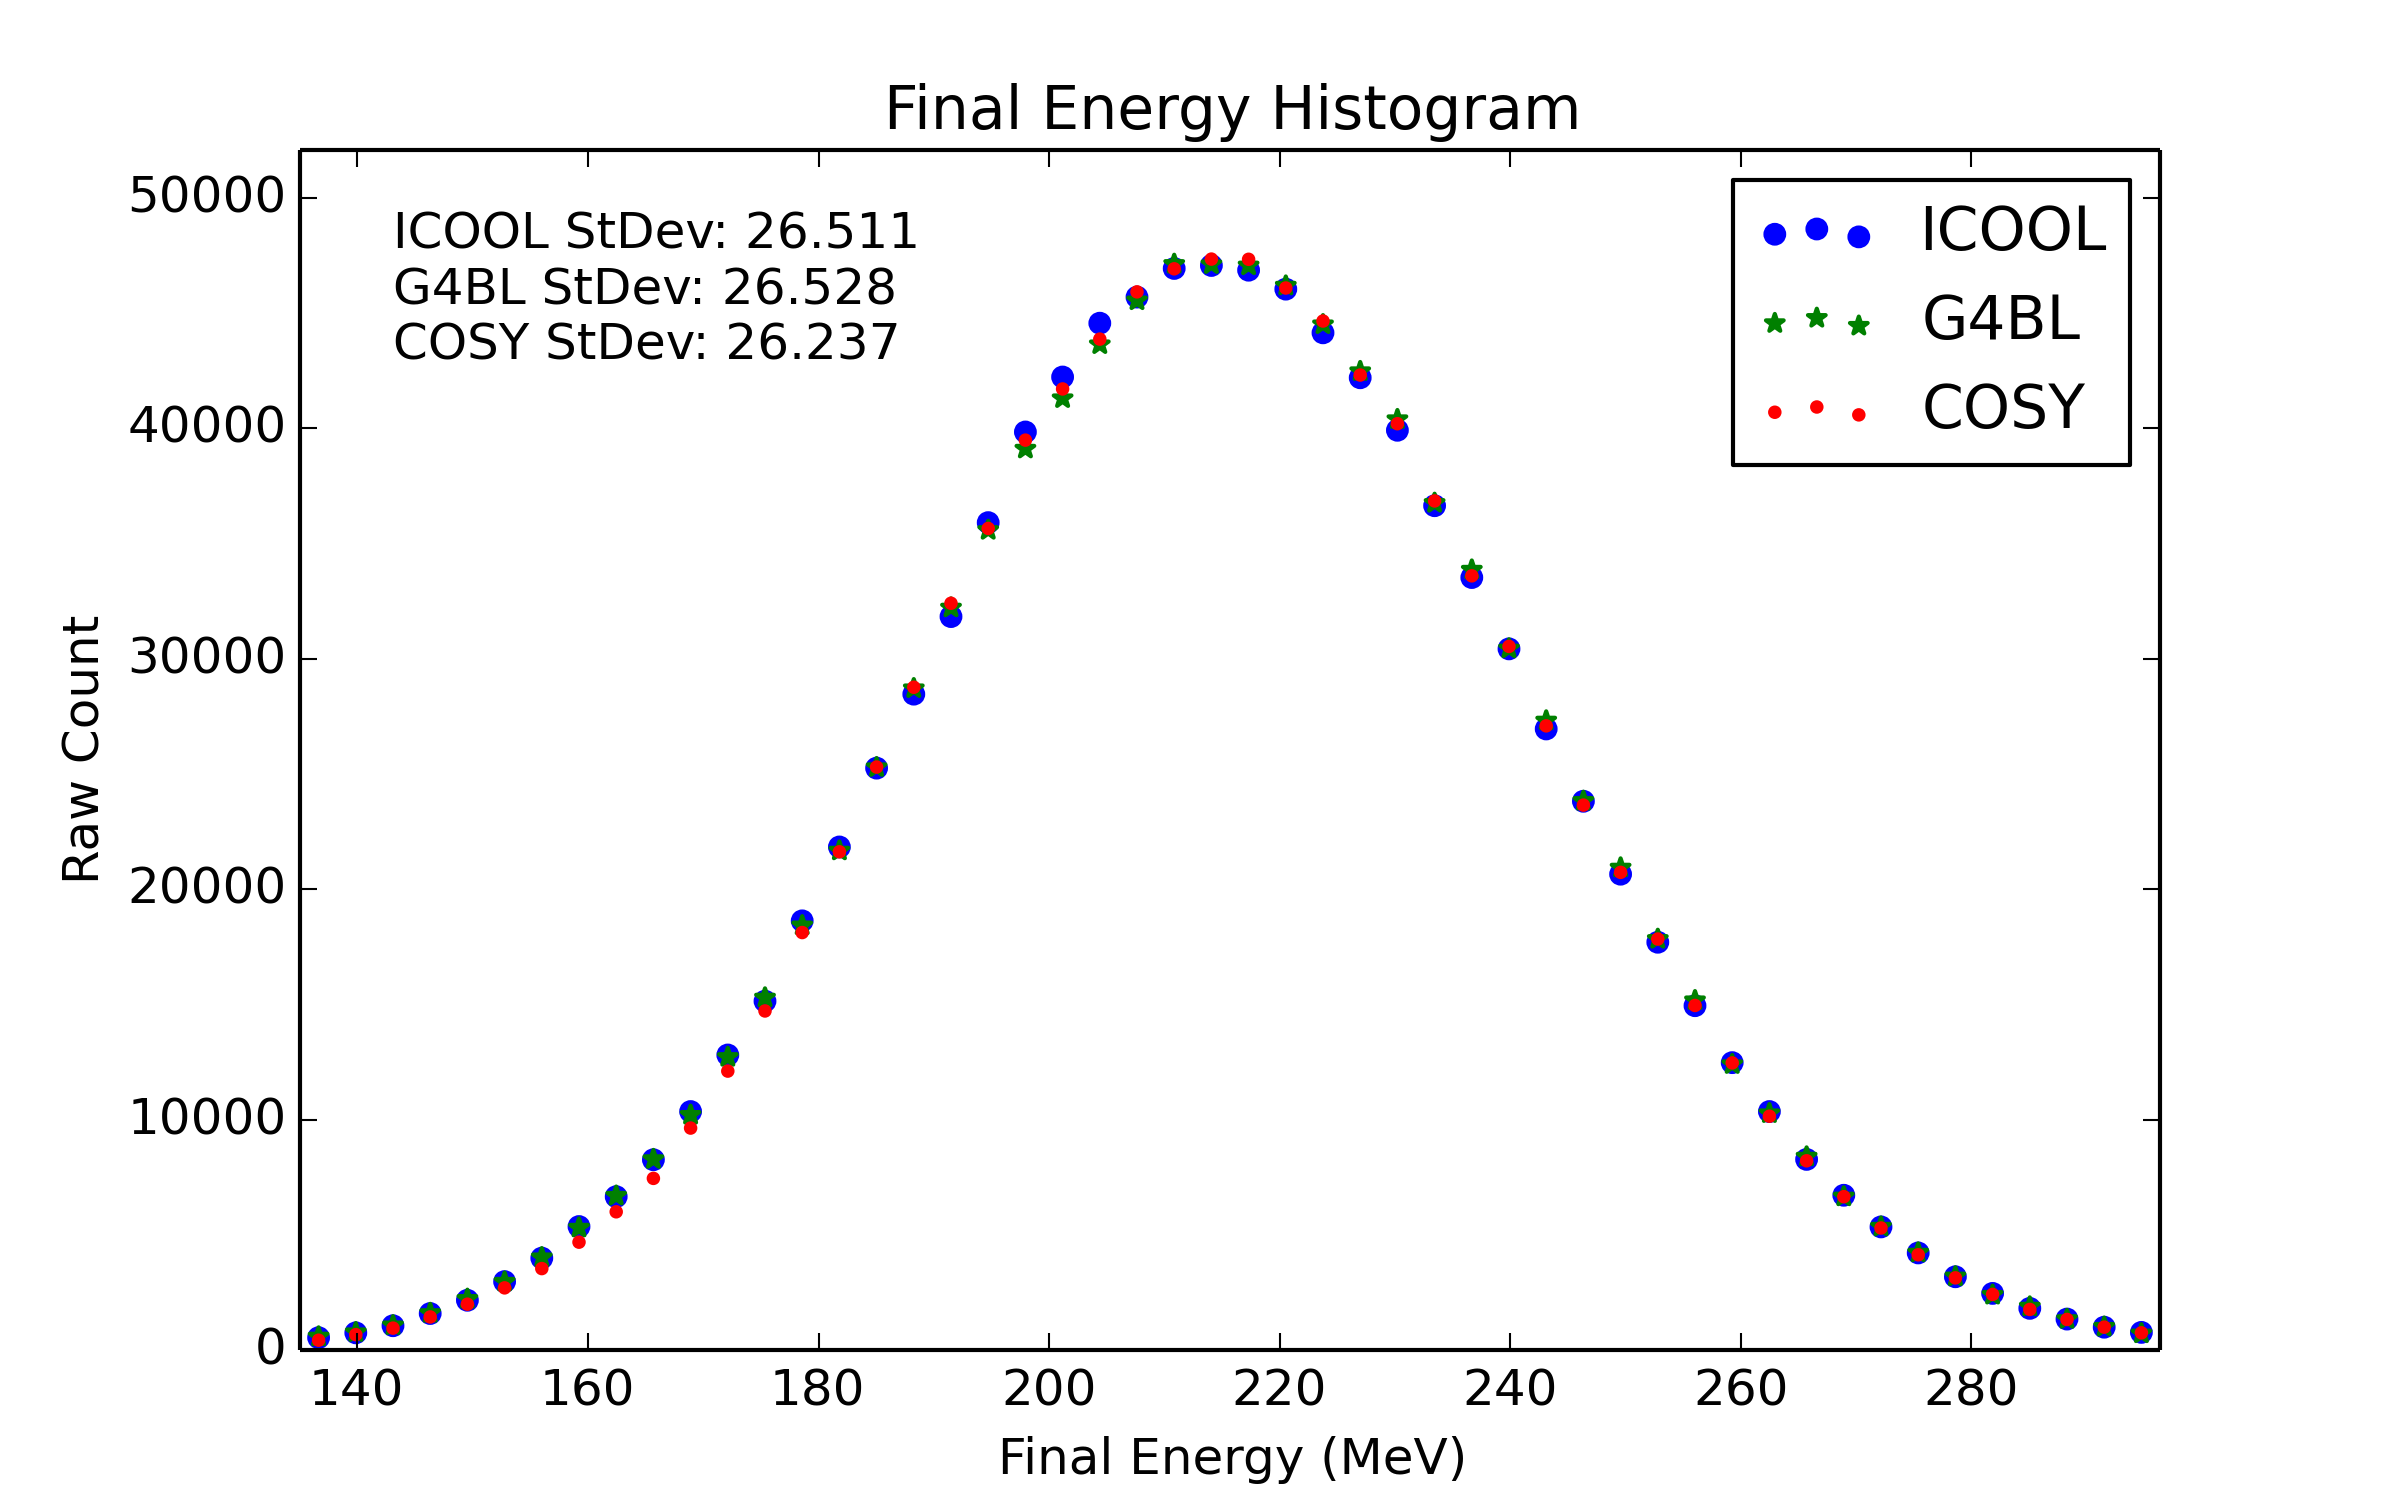
\includegraphics[width=\textwidth]{MICE data/LiH/e} 
  \caption{MICE Step IV final energy results for lithium hydride.}
  \label{fig:mice_lih_energy}
\end{figure}

\Subsection{Step Size Effects}\label{ssc:step_size_effects}
Several step sizes were tested in COSY to ensure optimal efficiency. While it was found that the results are fairly consistent regardless of step size, the results are discussed here.

For the upstream section ($-2.45105$ m to $-0.35/2$ m) of the MICE liquid hydrogen lattice, it was found that COSY operated sufficiently well at order 5 and with 100 steps in the simulation.

To study this step size dependence, $10^5$ particles from the initial distribution found in Table \ref{tbl:MICE_initial_distribution_parameters} were propagated through the upstream coils. Table \ref{tbl:mice_step_size_upstream} shows the effect of changing the step size for the upstream section. The step size in ICOOL was 1 mm and G4Beamline was left to its default step size.

\begin{table}
\caption*{\textbf{Step Size Dependence for Upstream Section}}
\begin{center}
\begin{tabularx}{\textwidth}{cccccc}
\hline \hline
Parameter & 3@50 & 3@100 & 5@100 & G4Beamline & ICOOL\\
\hline
$\sigma_x$ (mm): & 46.44 & 46.47 & 46.94 & 46.80 & 46.80\\
$\sigma_{\theta_x}$ (mrad): & 91.7 & 91.6 & 92.4 & 92.8 & 92.8\\
%$\sigma_y$ (mm): & 46.64 & 46.66 & 47.17 & 47.02 & 47.02\\
%$\sigma_{\theta_y}$ (mrad): & 92.1 & 92.0 & 92.8 & 93.1 & 93.1\\
Computational time (s): & 8.3 & 10.2 & 22.4 & 366 & 1353\\
\hline
\end{tabularx}
\end{center}
\caption[Step size dependence for the upstream section of the MICE Step IV lattice.]{Step size dependence for the upstream section of the MICE Step IV lattice. The notation for COSY is [order] @ [number of steps].}
\label{tbl:mice_step_size_upstream}
\end{table}

For all three COSY cases, the discrepancy w.r.t. G4Beamline is  $<$1\% for the transverse position component and on the order of 1\% for the angular component. 5th order at 100 steps was selected as ``best'' because of the increased agreement with both ICOOL and G4Beamline when compared to both 3@50 and 3@100. This is particularly true for the angular component. While 5@100 requires over double the computational time of 3@100, the computational time for 5@100 is still acceptable.

Results of the upstream simulation can be seen in Figures \ref{fig:upx} and \ref{fig:uppx}. There is good agreement between ICOOL, G4Beamline, and COSY. Note that ICOOL agrees with G4Beamline extremely well because ICOOL is using a field map generated by G4Beamline (as was discussed in Section \ref{ssc:miceResults}, the MICE results section).

\begin{figure}[H]
  \centering
    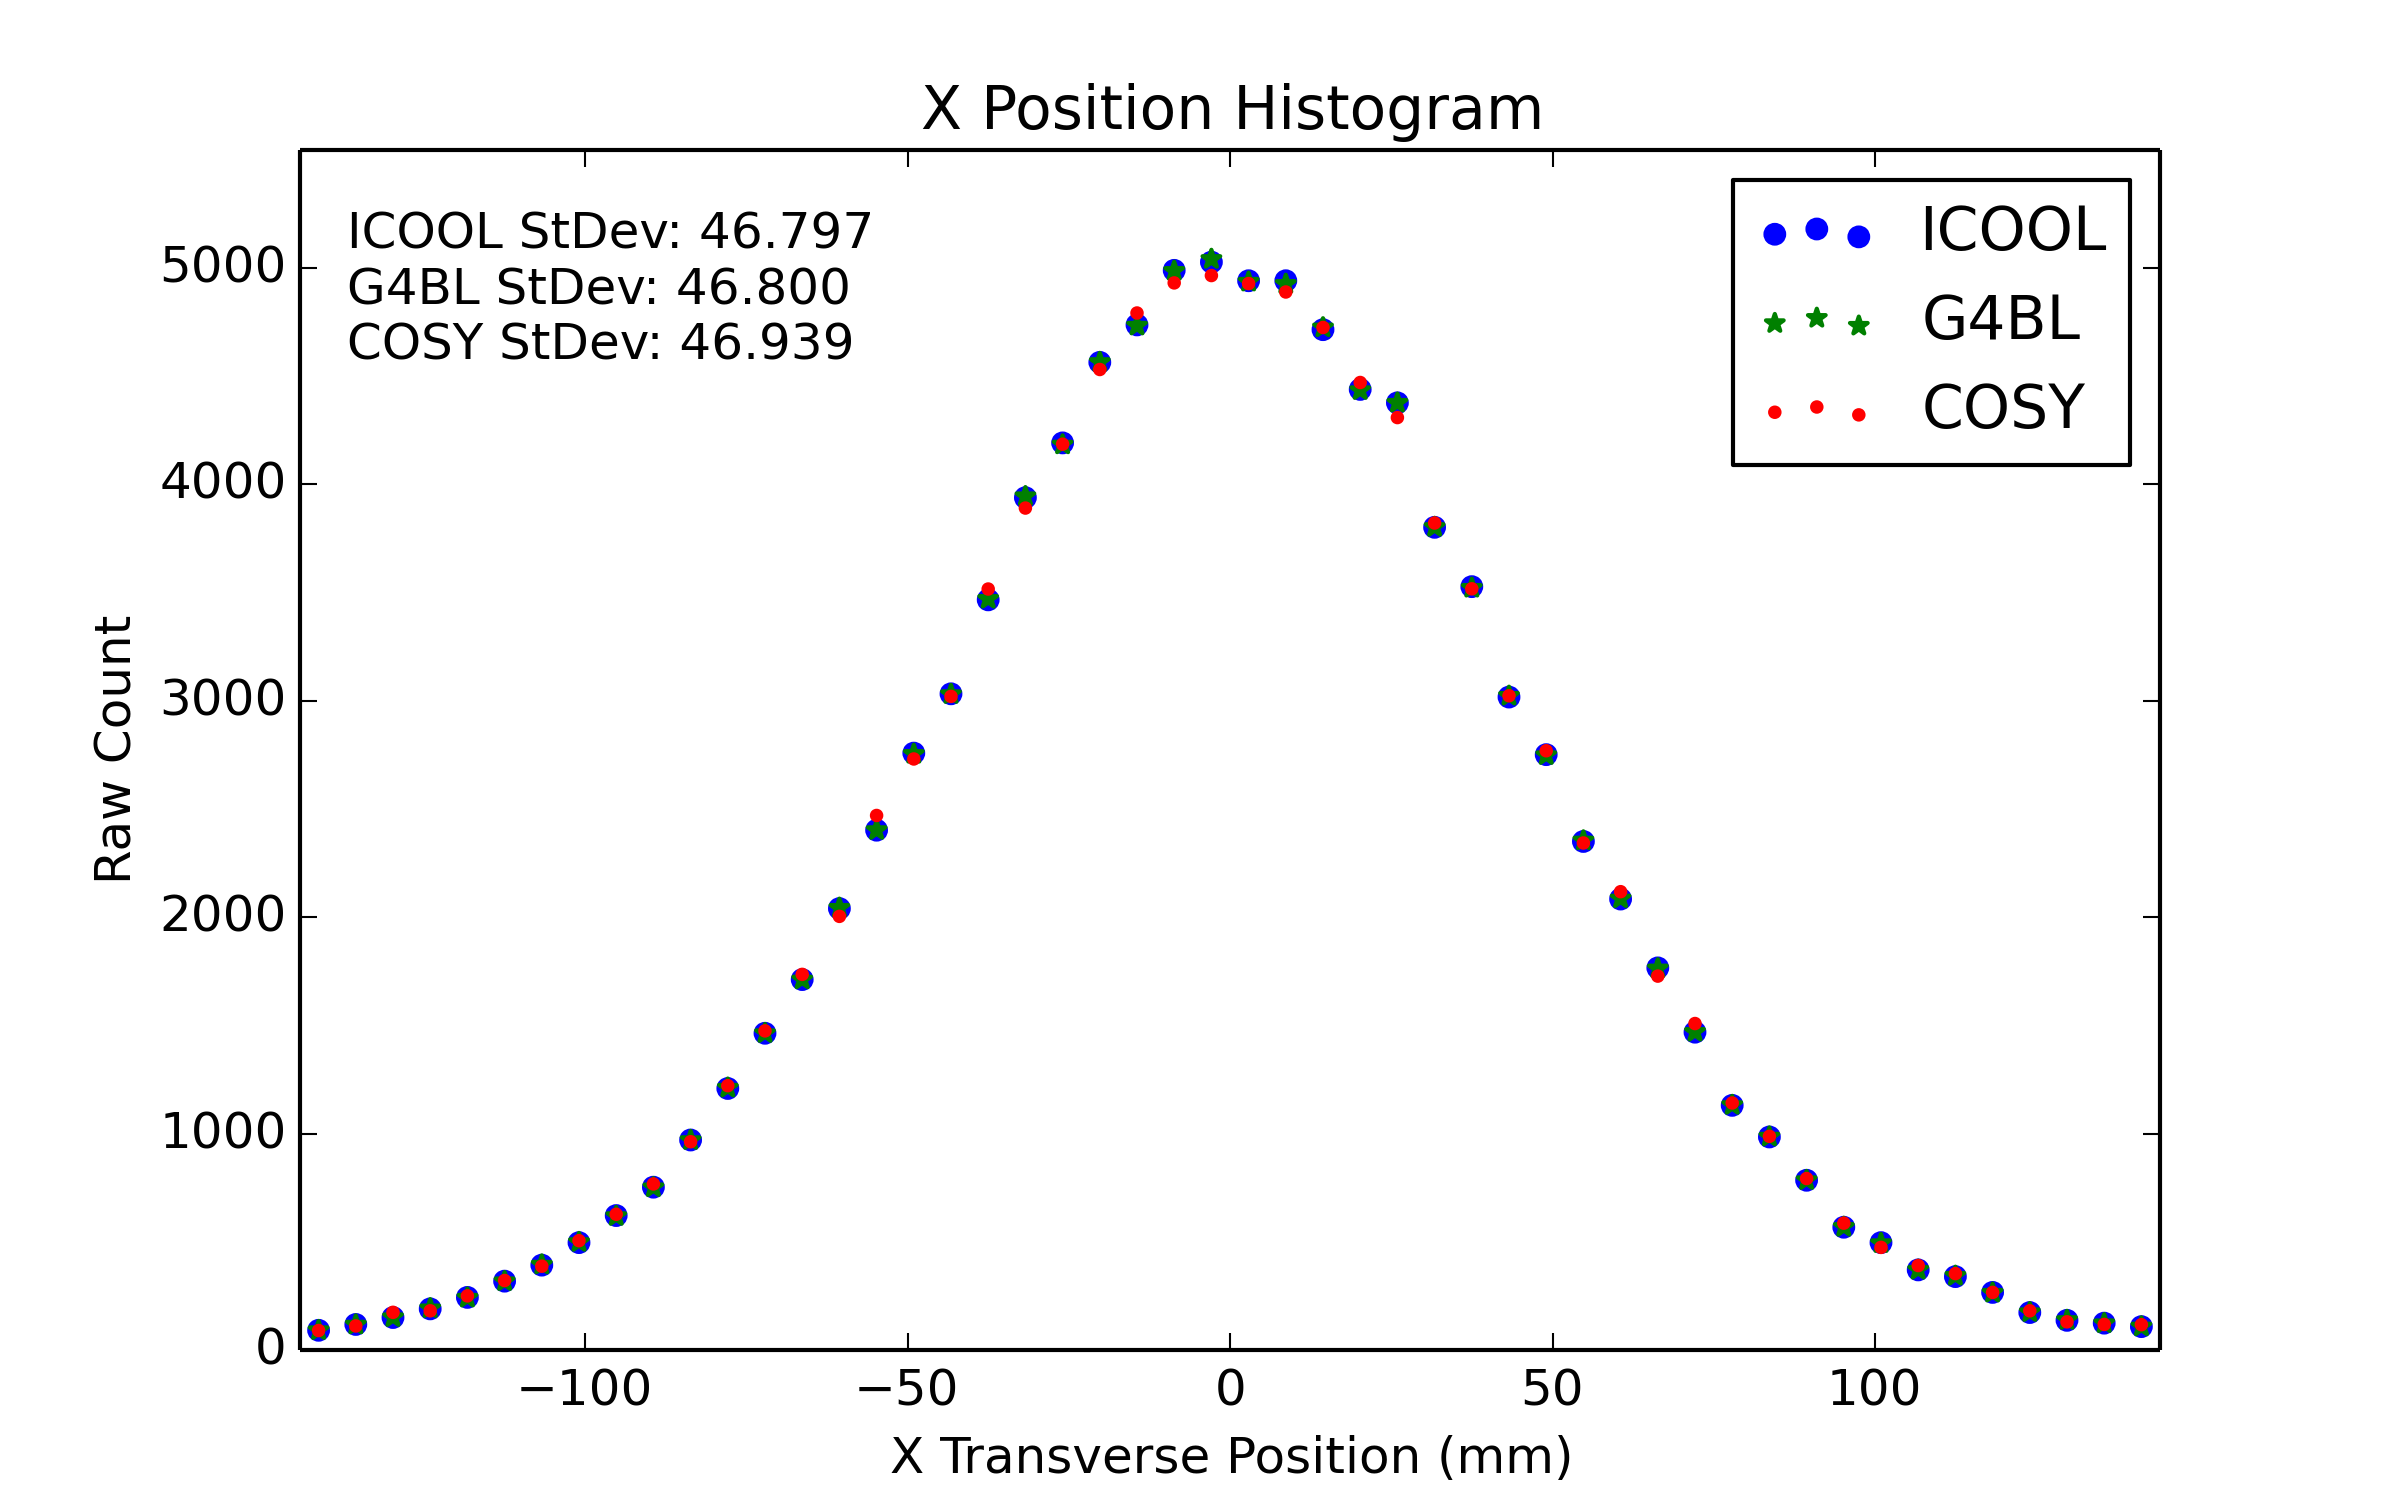
\includegraphics[width=0.7\textwidth]{MICE data/upstream/x} 
  \caption{Upstream simulation results for $x$ at 5th order and 100 steps.}
  \label{fig:upx}
\end{figure}

\begin{figure}[H]
  \centering
    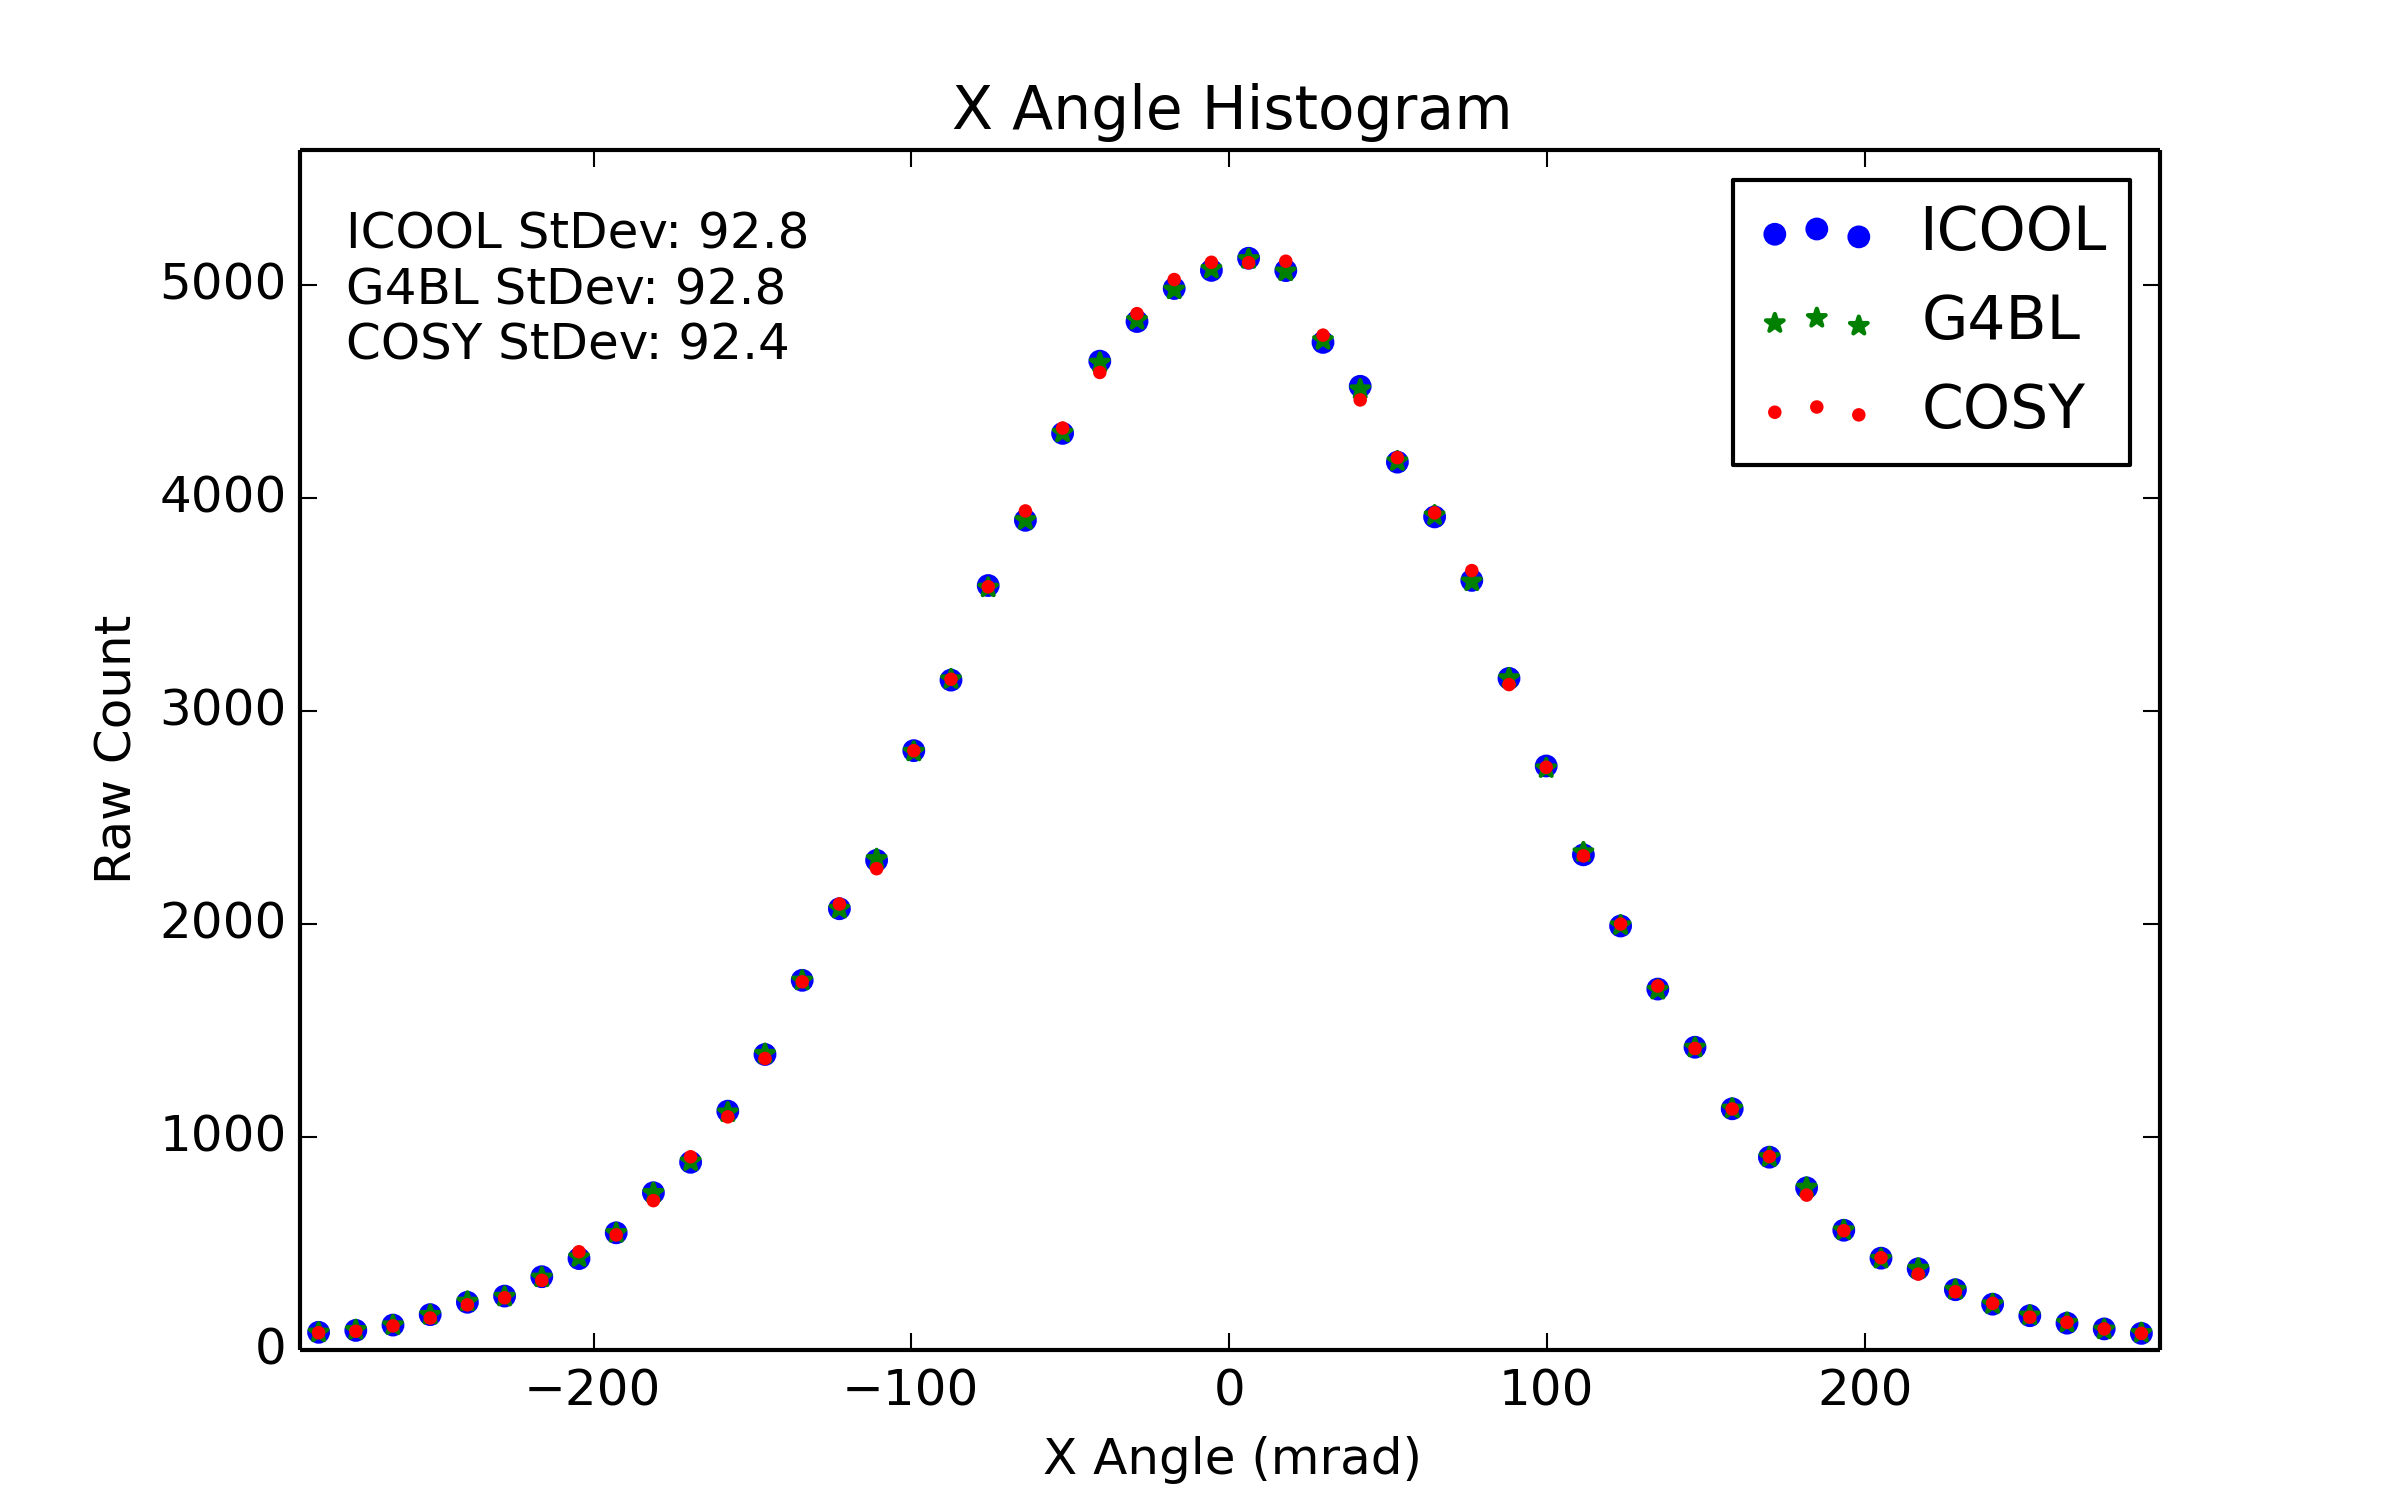
\includegraphics[width=0.7\textwidth]{MICE data/upstream/px} 
  \caption{Upstream simulation results for $\theta_x$ at 5th order and 100 steps.}
  \label{fig:uppx}
\end{figure}

For the absorber-coil section of the MICE liquid hydrogen lattice ($-$0.35/2 to 0.35/2), it was found that a 10 mm step size was sufficient to approximate the superposition of the absorber and coils. To study this step size dependence, $10^5$ particles from the initial distribution found in Table \ref{tbl:MICE_initial_distribution_parameters} were propagated through the 350 mm liquid hydrogen flat absorber. This simulation took the surrounding magnetic fields into account. Table \ref{tbl:mice_step_size_ac} shows the effect of changing the step size for the absorber-coil section only. The step size in ICOOL was 1 mm and G4Beamline was left to its default step size.

\begin{table}
\caption*{\textbf{Step Size Dependence for Absorber-Coil Section (Liquid Hydrogen)}}
\begin{center}
\begin{tabularx}{\textwidth}{cccccc}
\hline \hline
Parameter &1 mm & 10 mm & 50 mm & G4Beamline & ICOOL\\
\hline
$\sigma_x$ (mm): & 51.29 & 51.31 & 51.24 & 50.42 & 50.43\\
$\sigma_{\theta_x}$ (mrad): & 203.6 & 203.8 & 204.5 & 202.0 & 202.5\\
%$\sigma_y$ (mm): & 51.18 & 51.20 & 51.19 & 50.39 & 50.38\\
%$\sigma_{\theta_y}$ (mrad): & 203.0 & 203.2 & 203.8 & 201.9 & 202.4\\
$\sigma_E$ (MeV): & 26.66 & 26.66 & 26.64 & 26.67 & 26.67\\
Computational time (s): & 240.9 & 27.8 & 10.8 & 257.8 & 25.4\\
\hline
\end{tabularx}
\end{center}
\caption[Step size dependence for the absorber-coil section of the MICE Step IV lattice for liquid hydrogen.]{Step size dependence for the absorber-coil section of the MICE Step IV lattice for liquid hydrogen.}
\label{tbl:mice_step_size_ac}
\end{table}

The discrepancy of COSY w.r.t. G4Beamline is on the order of 1\% for the angular component and $<$1\% for the other components. Results of the absorber-coil simulation can be seen in Figures \ref{fig:acx}-\ref{fig:ace}. There is good agreement between ICOOL, G4Beamline, and COSY.

\begin{figure}[H]
  \centering
    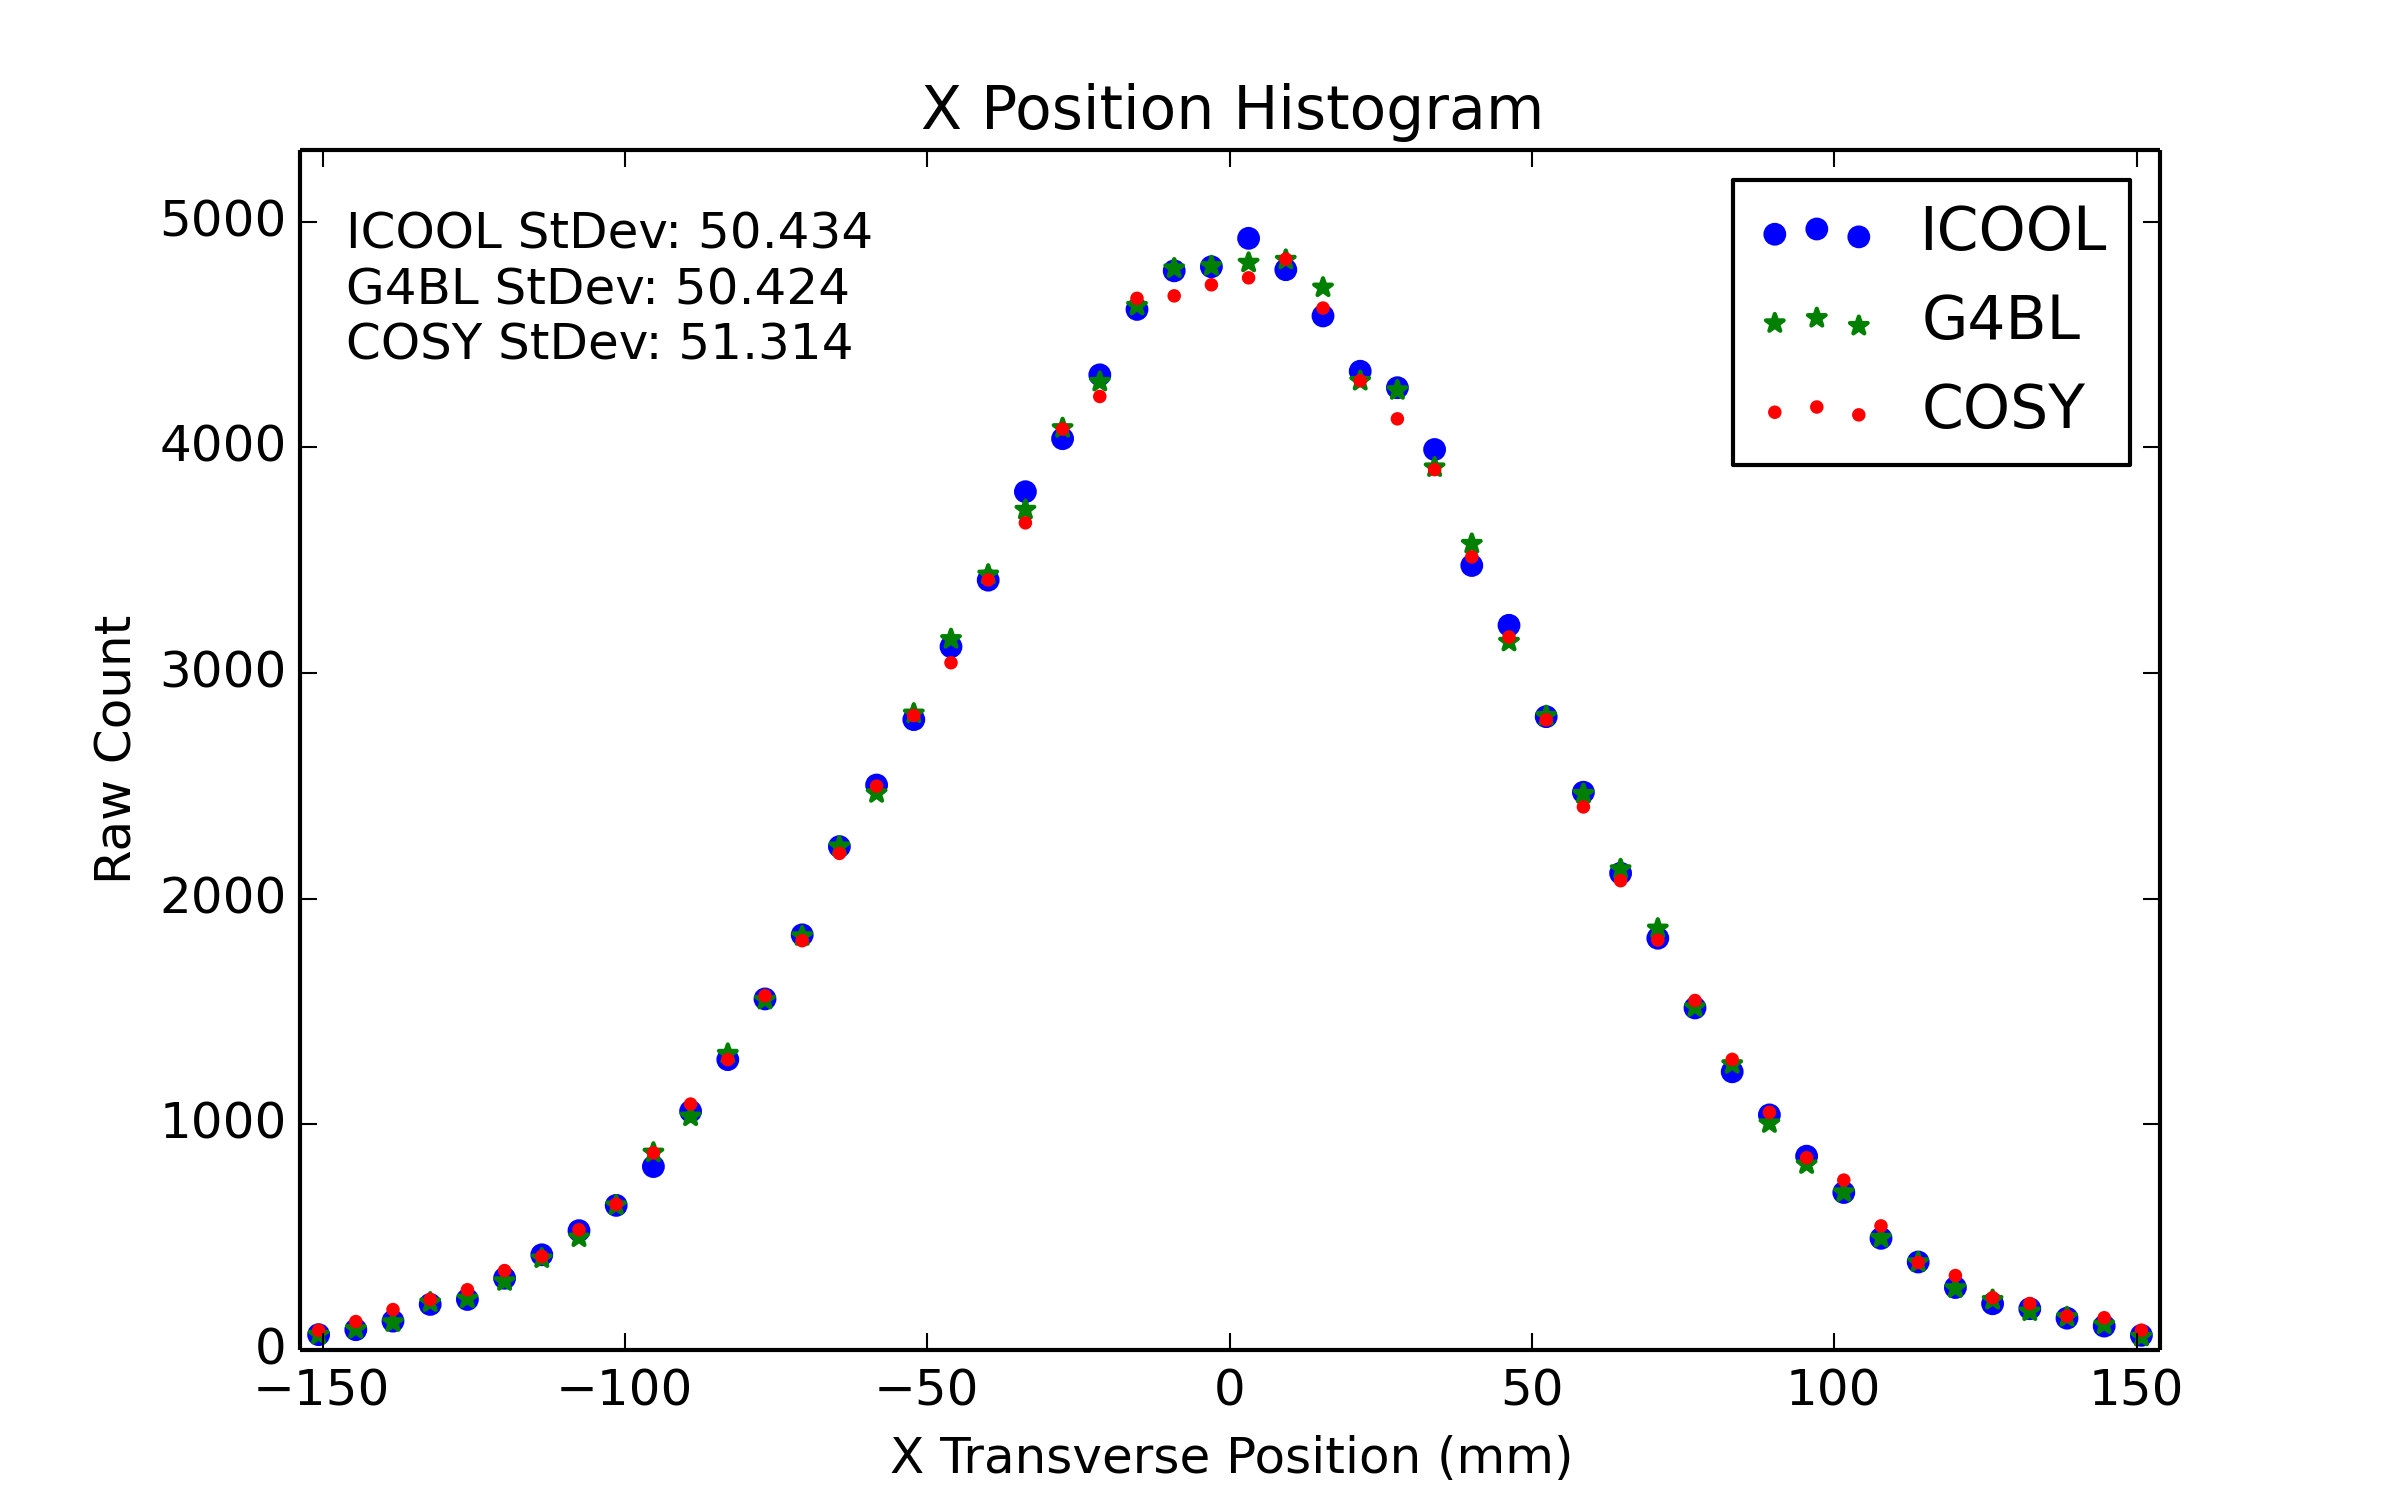
\includegraphics[width=0.7\textwidth]{MICE data/absorber coils/x} 
  \caption{Absorber-coil simulation results for $x$ at a step size of 10 mm.}
  \label{fig:acx}
\end{figure}

\begin{figure}[H]
  \centering
    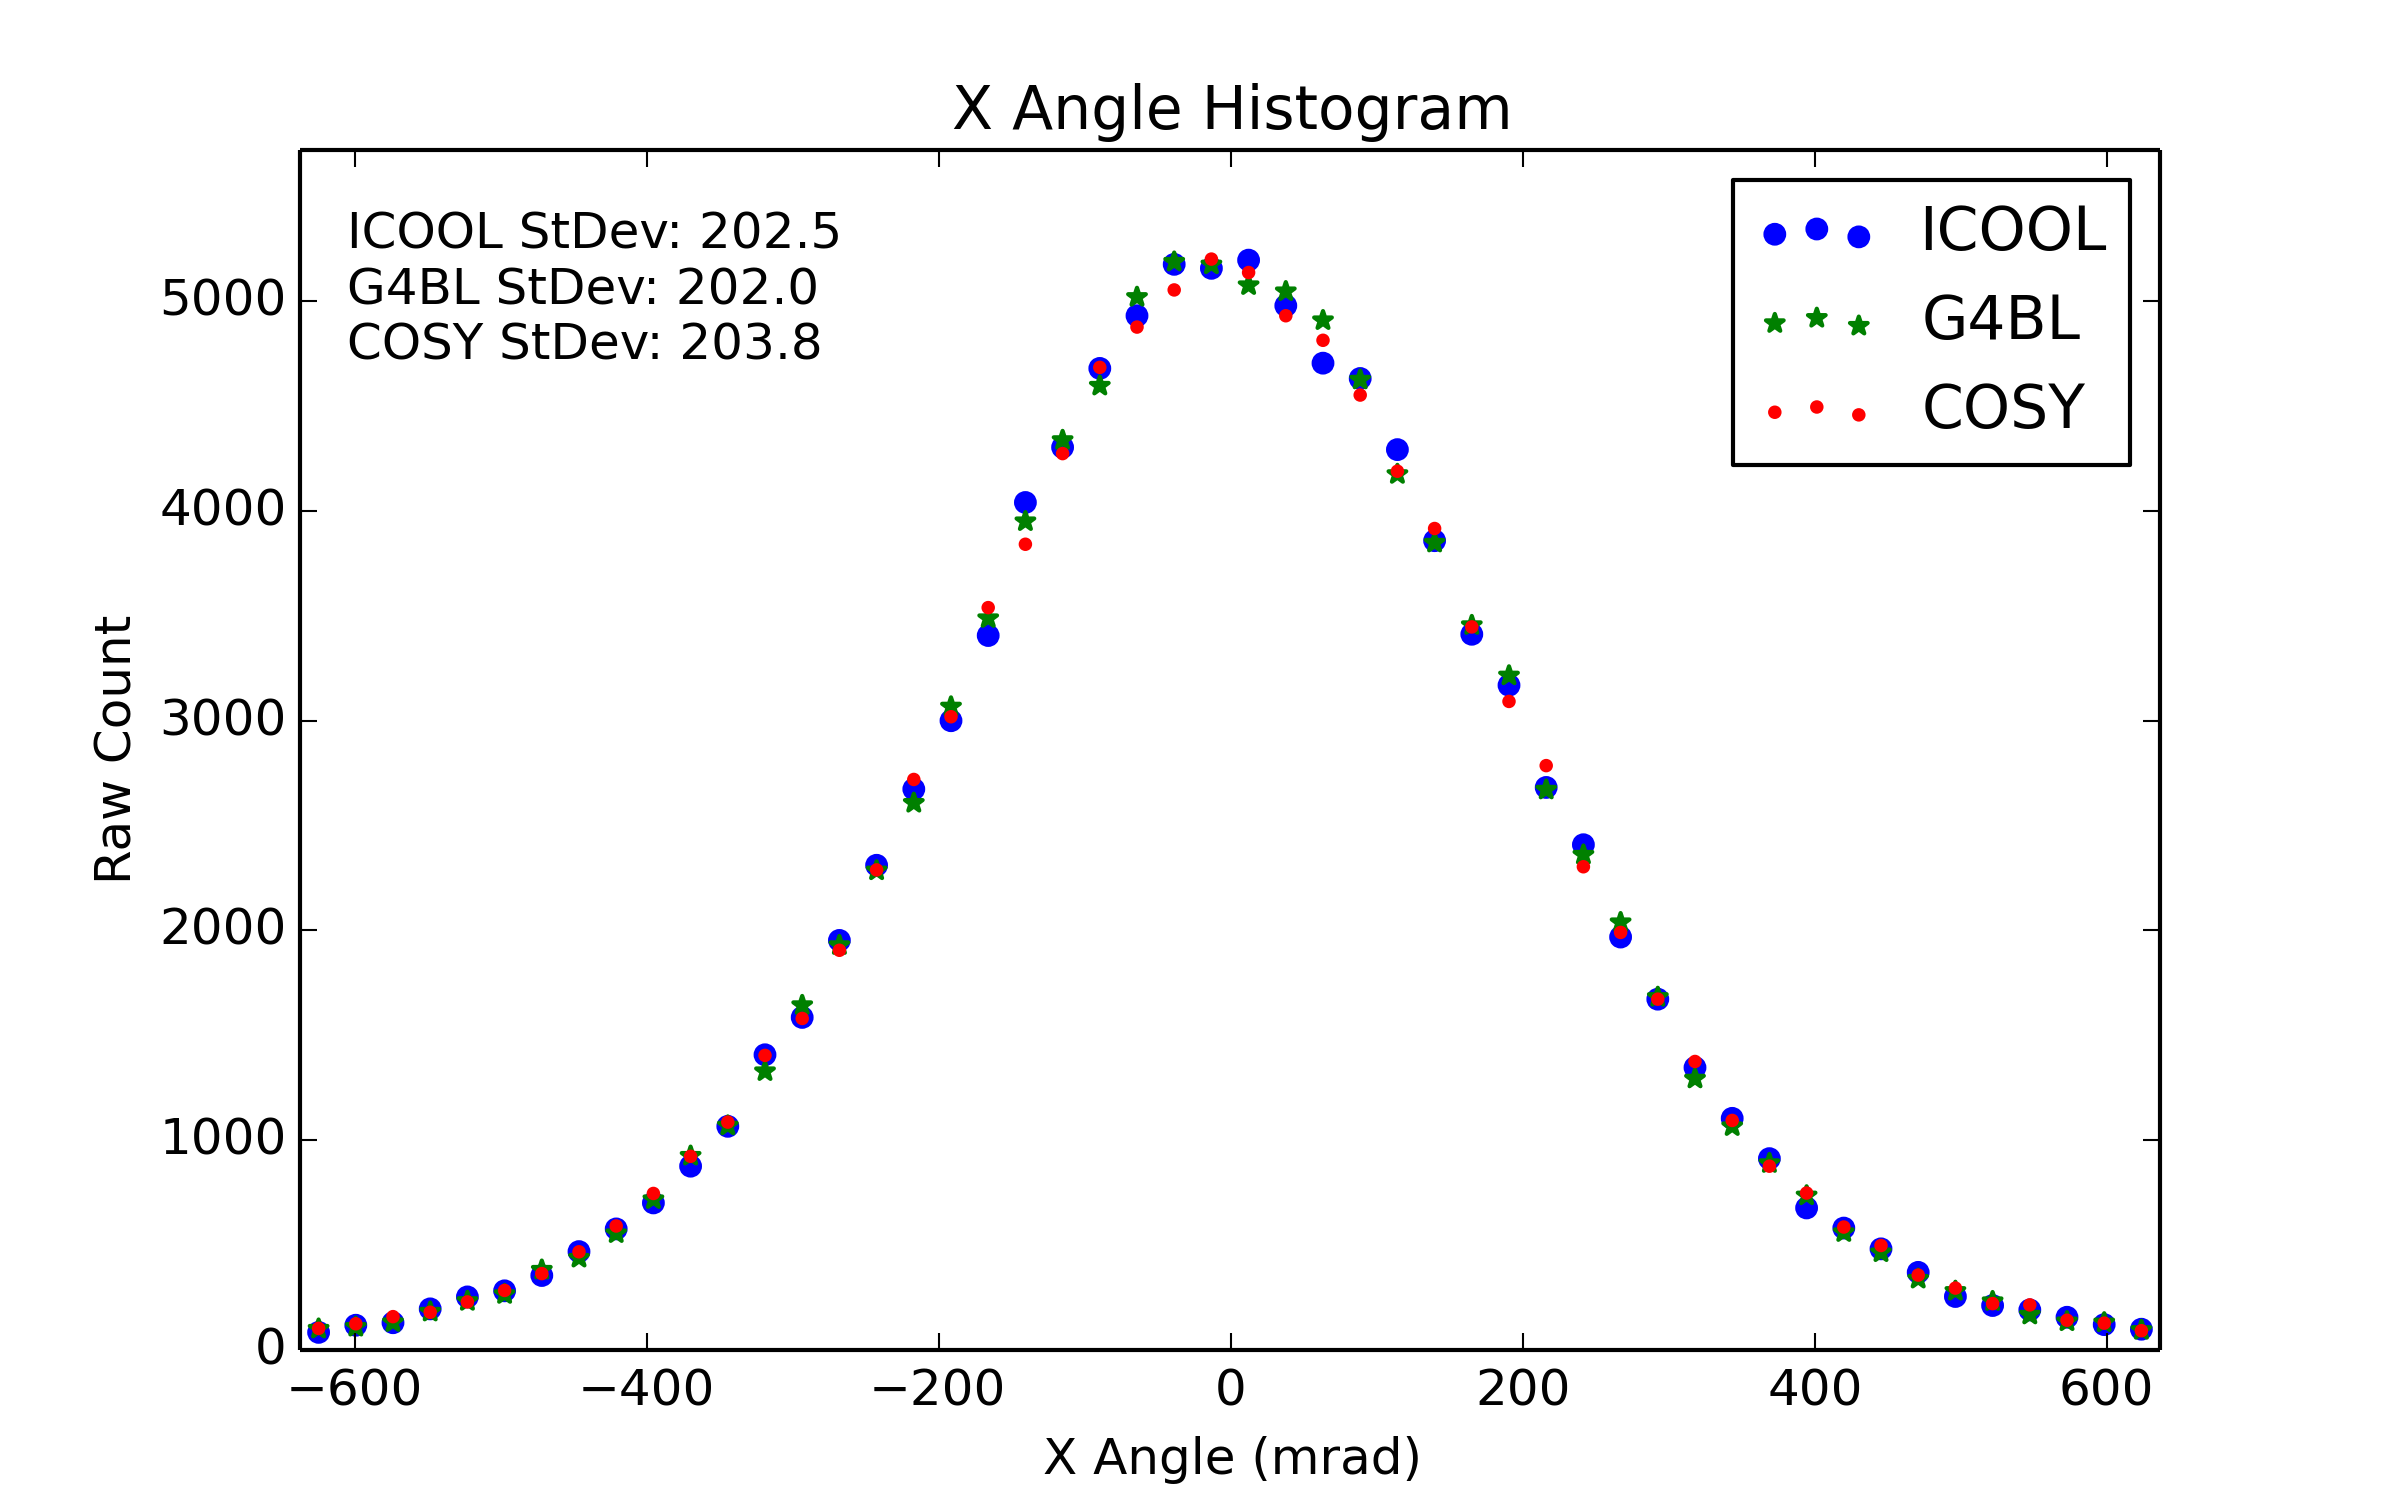
\includegraphics[width=0.7\textwidth]{MICE data/absorber coils/px} 
  \caption{Absorber-coil simulation results for $\theta_x$ at a step size of 10 mm.}
  \label{fig:acpx}
\end{figure}

\begin{figure}[H]
  \centering
    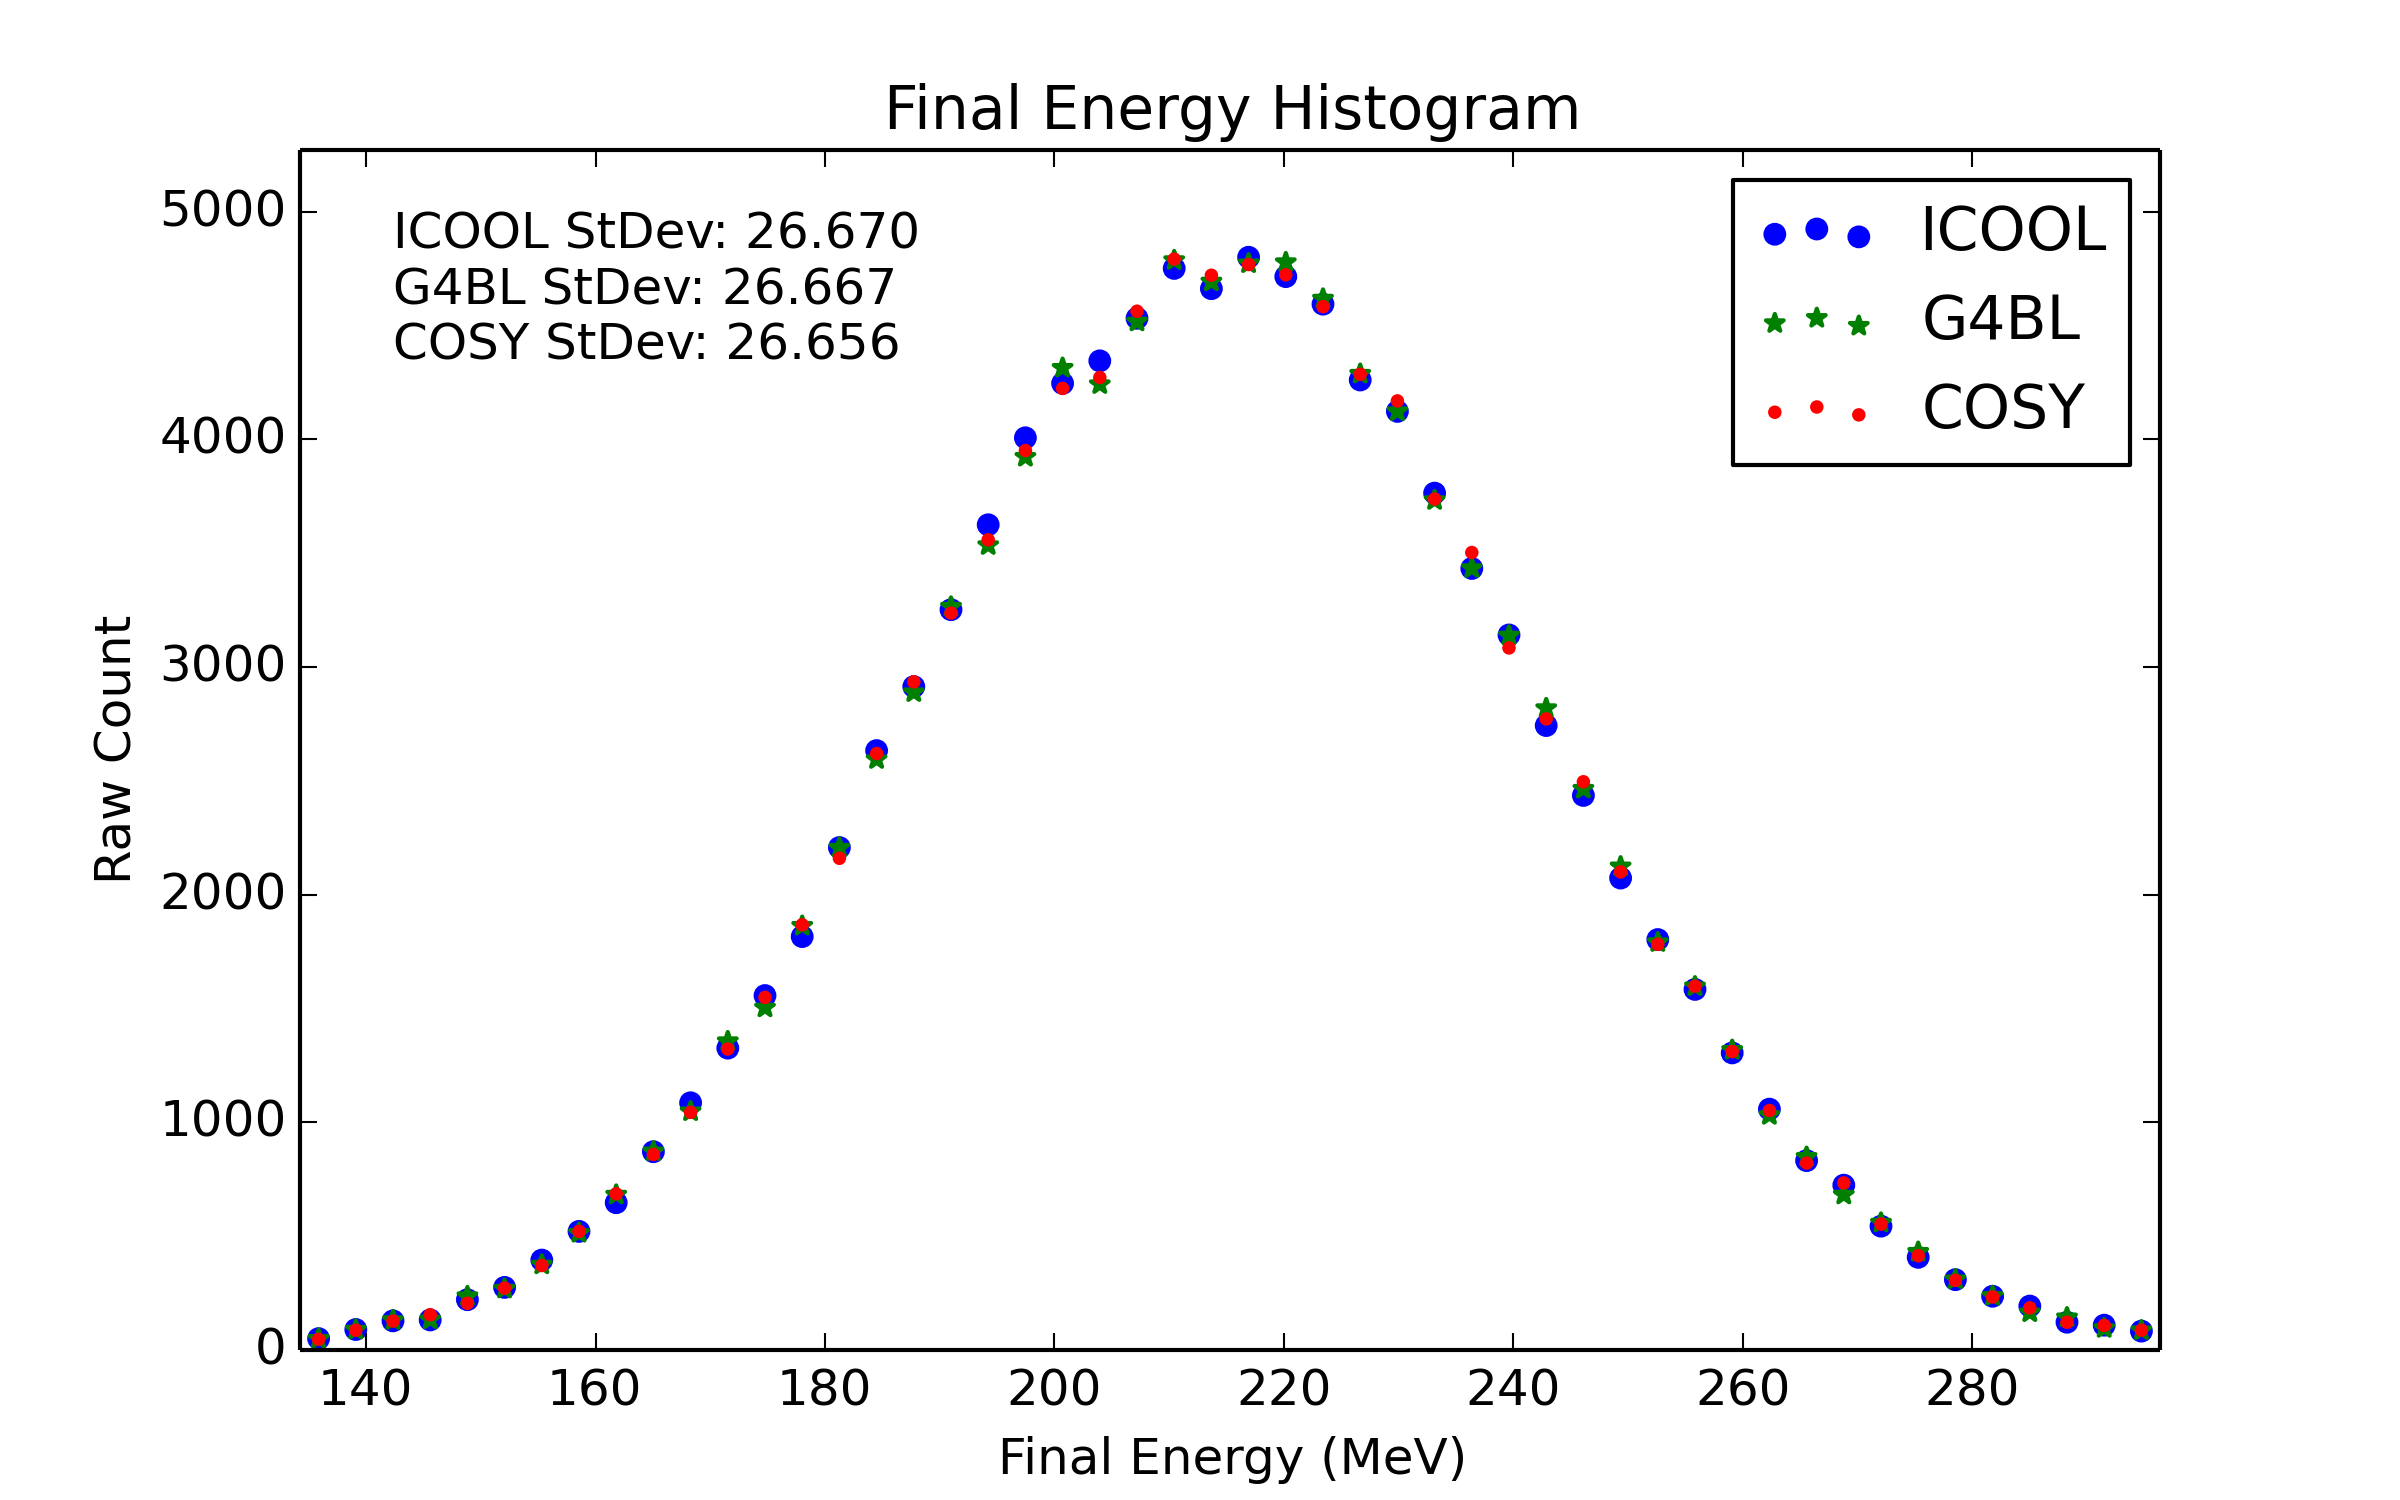
\includegraphics[width=0.7\textwidth]{MICE data/absorber coils/e} 
  \caption{Absorber-coil simulation results for the final energy at a step size of 10 mm.}
  \label{fig:ace}
\end{figure}

Since the downstream coils are very similar to the upstream coils, the downstream coils were not tested. For the full simulation in Section \ref{ssc:miceResults}, the downstream order and step size were identical to the upstream order and step size.

\Section{Code Implementation}\label{sec:code_implementation}

This section discusses in detail the organization and internal structure of the code. For reference, a reproduction of the code itself may be found in Appendix \ref{apx:code}. First, the user input will be discussed. Next, the \texttt{cosy.fox} level of the code will be examined. Finally, the structure of the FORTRAN code will briefly be considered. Figure \ref{fig:cosy_flowchart} will be referenced during these discussions.

In addition to the user's input file, COSY also uses a \texttt{cosy.fox} file. This file contains a plethora of global variables, functions, and routines which the user can access. However, \texttt{cosy.fox} can also be used to hide most of the complicated machinery from the user. For example, for this study the routines in \texttt{cosy.fox} transform the COSY coordinates $(x, a, y, b, \ell, d)$ into absolute coordinates $(x, p_x, y, p_y, t, E)$\footnote{Recall from Eqn. \ref{eqn:phaseSpaceVector} that $x$ and $y$ are the transverse coordinates; $a=p_x/p_0$; $b=p_y/p_0$; $\ell=-(t-t_0)v_0\gamma/(1+\gamma)$; $\delta=(K-K_0)/K_0$; $E$ is the total energy; $K$ is the kinetic energy; and the subscript $0$ denote the coordinate of the reference particle.}, and then relays the information to the FORTRAN code. Both the user file and the \texttt{cosy.fox} file are written in COSYScript, the programming language of COSY. 

\begin{figure}[!htb]
  \centering
    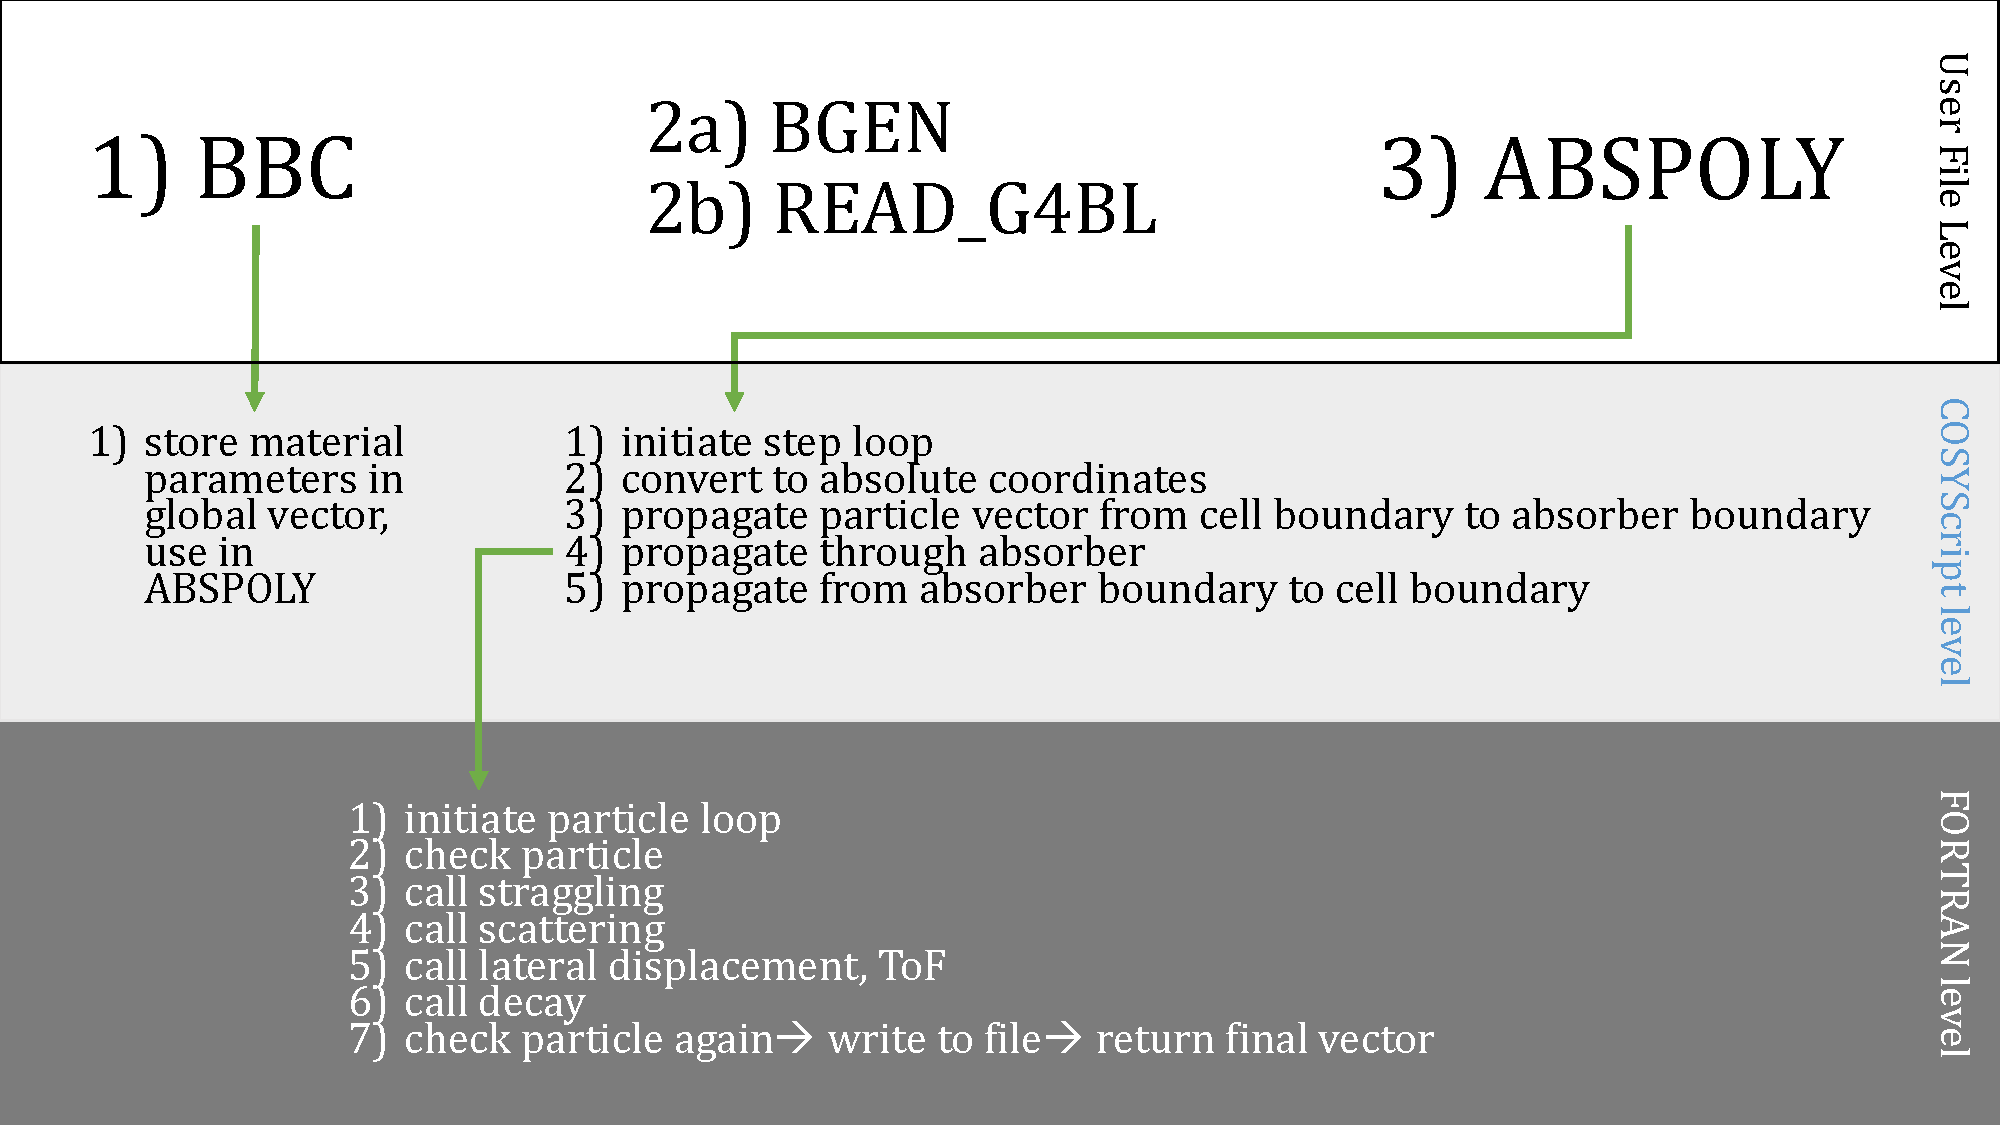
\includegraphics[width=\textwidth]{Figures/cosy_flowchart} 
  \caption{A flowchart for the structure of the new COSY routines implemented in this work.}
  \label{fig:cosy_flowchart}
\end{figure}

\Subsection{User Input}\label{ssc:user_input}
As with the deterministic absorber routine previously present in COSY, \texttt{WA}, the user must first call the procedure\\
\texttt{BBC} <$Z$> <$A$> <$\rho$> <$I$> <$\delta$> <$C$> \texttt{;} \\
This stores the material parameters in a global array. The arguments are the nuclear charge $Z$, the atomic mass $A$, the density of the material $\rho$, the ionization energy $I$, the density correction $\delta$, and the shell correction $C$. Next, the user must either generate a distribution of particles or read a distribution of particles from a file. Using \\
\texttt{BGEN} <$n$> <$V$> <$\mu_x$> <$\sigma_x$> <$\mu_{p_x}$> <$\sigma_{p_x}$> <$\mu_y$> <$\sigma_y$> <$\mu_{p_y}$> <$\sigma_{p_y}$> <$\mu_t$> <$\sigma_t$> <$\mu_{p_z}$> <$\sigma_{p_z}$> \texttt{;}\\
the user can generate a Gaussian beam of $n$ particles into a 2D vector $V$. Alternatively, the user may use \\
\verb|READ_G4BL| <\texttt{file}> <$n$> <$V$> \texttt{;}\\
to read a G4Beamline-formatted file of $n$ particles and store it into a vector $V$. Finally, the user can call\\
\texttt{ABSPOLY} <$S_1$> <$S_2$> <$n$> <$L$> <$A$> <$V$> <$X_0$> <$S_n$> <$L_c$> <$O$> \texttt{;}\\
where $S_1$ is an $n^{th}$ order polynomial describing the entrance surface, $S_2$ is an $n^{th}$ order polynomial describing the exit surface, $L$ is the on-axis length of the absorber, $A$ is the aperture, $V$ is the 2D input and output particle vector, $X_0$ is the radiation length of the material, $S_n$ is the number of steps inside the absorber, $L_c$ is the length of the absorber cell, and $O$ is the output save number (e.g. ``12'' to save the results in \texttt{fort.12}). A depiction of the parameters can be found in Figure \ref{fig:abspoly}.

\begin{figure}[!htb]
  \centering
    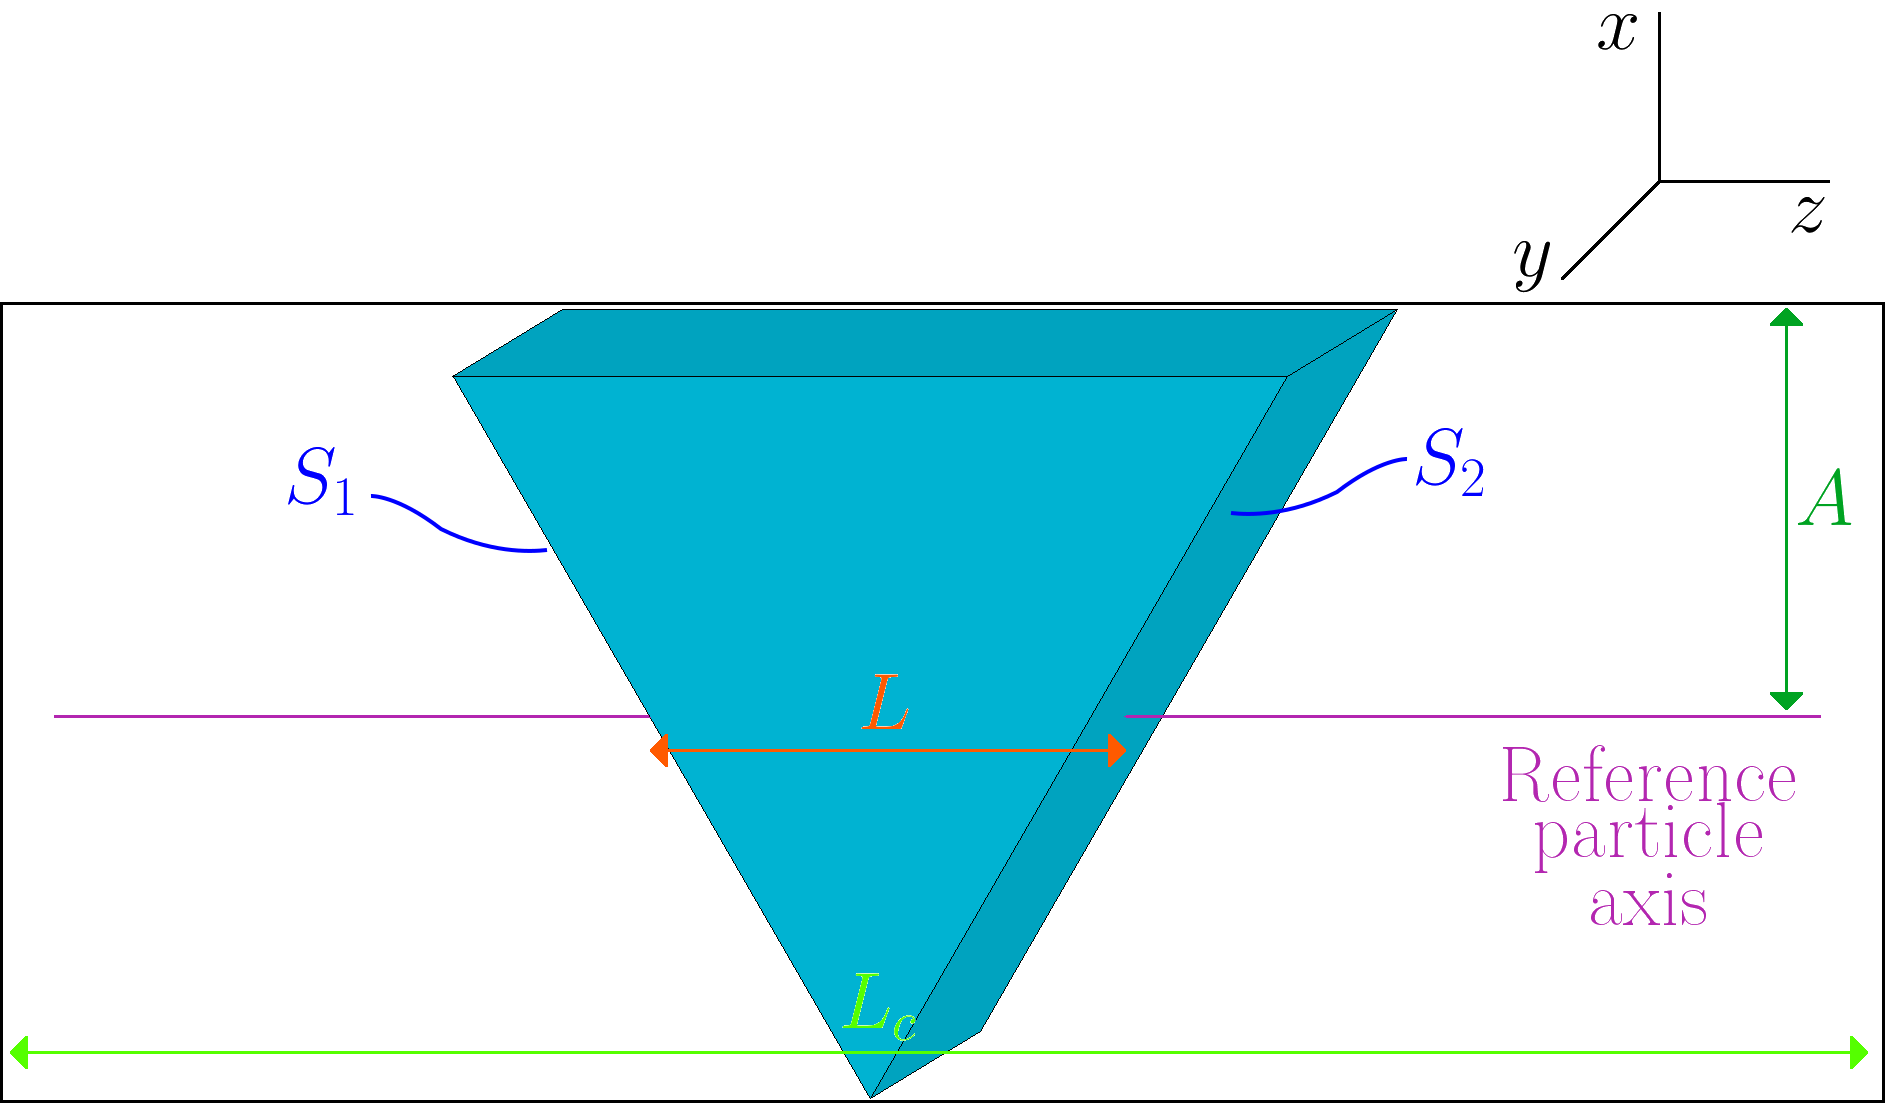
\includegraphics[width=\textwidth]{Figures/abspoly} 
  \caption{Cartoon example of some of the \texttt{ABSPOLY} parameters.}
  \label{fig:abspoly}
\end{figure}

\Subsection{COSYScript Level}\label{ssc:cosyscript}

As previously mentioned, the \texttt{ABSPOLY} routine is defined in the external file \texttt{cosy.fox}. Here, the step loop over $S_n$ is initialized. Next, the coordinates of the input 2D vector $V$ are converted from coordinates relative to the reference particle to absolute coordinates. The particle vector is then propagated from the cell boundary (whose width is defined by $L_c$) to the absorber (whose on-axis width is defined by $L$). If $L_c<L$ then no propagation occurs. When the particles are at the absorber boundary, the 2D particle vector $V$ is passed on to the FORTRAN level of the code, where propagation through the absorber takes place. The routine linking the COSYScript and FORTRAN levels is \texttt{STOABS} and will be discussed in Section \ref{ssc:fortran}. After the 2D particle vector $V$ is returned, $V$ is propagated to the end of the cell and returned to the user.

\Subsection{FORTRAN Level}\label{ssc:fortran}
Except for the propagation of particles through the absorber, the processes found in Section \ref{ssc:cosyscript} are much faster in COSYScript than in FORTRAN. This is because processes like coordinate conversion, propagation through a vaccum, etc. are deterministic and can therefore be handled by transfer maps.

The routine\\
\texttt{STOABS} <$V$> <$m$> <$L$> <$MP$> <$X_0$> <$O$> <$A$> <$n$> \texttt{;} \\
takes input parameters from the COSYScript level and returns the input 2D particle vector $V$. Here, $m$ is the particle mass (taken from the reference particle), $L$ is an $n$-dimentionial array containing the path lengths for each particle, $MP$ is an array containing the material parameters (taken from the global array $BETHEBLOCHC$ set up by the routine \texttt{BBC}), $X_0$ is the radiation length of the material, $O$ is the output save number, $A$ is the aperture, and $n$ is the number of particles.

Once the FORTRAN level has this information, a loop over $n$ particles is started. Each particle is checked at the beginning of each loop for the following flags: particle stopped, particle hit aperture, particle missed absorber, drift. If either the particle was stopped ($E\leq m$) or the particle hit the aperture ($x^2+y^2>=A^2$) then the particle is terminated. If the particle missed the absorber completely then the drift flag is turned on. If the drift flag is on then the particle is simply propagated without the stochastic processes called.

Provided that the particle has not been flagged, the particle is subject to energy straggling and then multiple scattering. After these two routines, the lateral displacement and time-of-flight corrections are called. It should be noted that the order matters for energy straggling and multiple scattering. The order does not matter for lateral displacement and time-of-flight provided that both straggling and scattering have already occurred. Finally, decay can be called. Note that for this work, decay has been turned off completely, and so this step is skipped.

Finally, the particle is checked again. If the output save number $O$ is not equal to zero then the particles are written to a file. Lastly, the 2D particle vector $V$ is returned to the COSYScript level.

\Section{Summary}\label{sec:summary}

In summary, new simulation tools for muon ionization cooling have been added to COSY Infinity for particle-by-particle propagation. The energy straggling, multiple scattering, transverse position, and time-of-flight models were developed from first principles. The algorithms implemented have been modified via empirical fit to MuScat \cite{muscat} while keeping reasonable agreement with G4Beamline. Fitted with this new software, COSY has simulated one of the current muon ionization cooling efforts, MICE Step IV \cite{mice}, yielding good agreement with both ICOOL and G4Beamline. The code developed in this work is accurate, fast, and user-friendly.